\documentclass[prl,onecolumn,lengthcheck]{revtex4-2}

\usepackage{amssymb, amsmath, amsthm, amstext, amsfonts, amsopn, amscd}

\usepackage{color}
\usepackage{xcolor}
\usepackage[colorlinks=true, linkcolor=black, breaklinks=true, citecolor=blue, urlcolor=red]{hyperref} 
\usepackage{times}
\usepackage{mathdots}
\usepackage{graphicx}
\usepackage{tikz}
\usepackage{pgfplots}
\usetikzlibrary{decorations.markings}
\usetikzlibrary{decorations.pathreplacing,calligraphy}

%\usetikzlibrary{external}
%\tikzexternalize

\definecolor{spacecadet}{HTML}{0D284C}
\definecolor{munsell}{HTML}{008FA8}
\definecolor{banana}{HTML}{FFD932}
\definecolor{cgblue}{HTML}{007CA5}
\definecolor{isabelline}{HTML}{EAEDEA}

% The preamble here sets up a lot of new/revised commands and
% environments.  It's annoying, but please do *not* try to strip these
% out into a separate .sty file (which could lead to the loss of some
% information when we convert the file to other formats).  Instead, keep
% them in the preamble of your main LaTeX source file.


% The following parameters seem to provide a reasonable page setup.

%\topmargin 0.0cm
%\oddsidemargin 0.2cm
%\textwidth 16cm 
%\textheight 21cm
%\footskip 1.0cm


%The next command sets up an environment for the abstract to your paper.

%\newenvironment{sciabstract}{%
%\begin{quote} \bf}
%{\end{quote}}


\newcommand{\tr}{\operatorname{tr}}
\newcommand{\Tr}{\operatorname{Tr}}

\newcommand{\cA}{\mathcal A}\newcommand{\scrA}{\mathscr A}\newcommand{\fA}{\mathfrak A}
\newcommand{\ua}{\textup a}
\newcommand{\cB}{\mathcal B}\newcommand{\scrB}{\mathscr B}\newcommand{\fB}{\mathfrak B}
\newcommand{\C}{\mathbb{C}}
\newcommand{\cD}{\mathcal D}
\newcommand{\ud}{\textup d}
\newcommand{\cE}{\mathcal E}
\newcommand{\fF}{\mathfrak{F}}\newcommand{\cF}{\mathcal{F}}\newcommand{\sF}{\mathscr{F}}
\newcommand{\fg}{\mathfrak g}
\newcommand{\scrh}{\mathscr h}\newcommand{\fh}{\mathfrak h}
\newcommand{\cH}{\mathcal H}\newcommand{\fH}{\mathfrak H}\newcommand{\scrH}{\mathscr H}
\newcommand{\ltwo}{\ell^{2}}
\newcommand{\N}{\mathbb{N}}
\newcommand{\fP}{\mathfrak{P}}
\newcommand{\R}{\mathbb{R}}\newcommand{\cR}{\mathcal R}
\newcommand{\T}{\mathbb{T}}
\newcommand{\fu}{\mathfrak{u}}
\newcommand{\Z}{\mathbb{Z}}

\newcommand{\1}{\mathds{1}}

\newcommand{\vep}{\varepsilon}
\newcommand{\vth}{\vartheta}
\newcommand{\vp}{\varphi}


\begin{document} 

\title{Quantum Simulation of Conformal Field Theory} 

\author{Tobias J.\ Osborne$^{1}$ and Alexander Stottmeister$^{1}$}

\affiliation{$^{1}$Institut f\"ur Theoretische Physik, Leibniz Universit\"at Hannover, Appelstr. 2, 30167 Hannover, Germany}

\begin{abstract}
We discuss a novel approach to the quantum simulation of 1+1-dimensional conformal field theory (CFT) invoking the framework of operator-algebraic renormalization. A given CFT is treated in terms of effective lattice field theories appropriate to observational scales. Discretization of continuum quantities is controlled via the renormalization group leading to rigorous and provable error bounds. Explicitly, we discuss free fermion CFTs with central charge $c=\tfrac{1}{2}$ in the Ramond and Neveu-Schwarz sector as the basis of Ising CFTs and Wess-Zumino-Witten currents. A full error analysis in this case suggests near-term applicability: promising results are obtained already with $128$ logical qubits.
\end{abstract}

\maketitle 

\paragraph*{Introduction.} 
Understanding quantum field theory (QFT)
is a central open problem in theoretical physics, with unique challenges arising from the infinite number of degrees of freedom to the possibility of large quantum entanglement \cite{douglasFoundationsQuantumField2012,seibergNathanSeiberg20152014,wittenAPSMedalExceptional2018}.
With the imminent advent of scalable fault-tolerant quantum computation a new era in the understanding of strongly interacting many body systems via \emph{quantum simulation} \cite{feynmanSimulatingPhysicsComputers1981,lloydUniversalQuantumSimulators1996,abramsSimulationManyBodyFermi1997a,zalkaSimulatingQuantumSystems1998}
becomes possible, with a slew of recent realisations \cite{smithSimulatingQuantumManybody2019,zhangObservationManybodyDynamical2017,bernienProbingManybodyDynamics2017},
enabling breakthrough quantum algorithms for scattering events in QFT \cite{jordanQuantumAlgorithmsQuantum2012,hamedmoosavianFasterQuantumAlgorithm2018,jordanQuantumAlgorithmsFermionic2014,preskillSimulatingQuantumField2018}. Following Wilson \cite{wilsonRenormalizationGroupCritical1975,wilsonRenormalizationGroupCritical1983,wilsonRenormalizationGroupEpsilon1974},
the results are interpreted in \emph{effective field theory} supplying predictions appropriate for the energy scale -- the \emph{renormalization scale} -- set by the lattice spacing. The consistency under changes of scale gives the definition of an ultraviolet completion -- a procedure known as the renormalization group
\cite{durrInitioDeterminationLight2008,creutzQuarksGluonsLattices1985}. However, effective field theory does not provide us with all the answers. In particular, \emph{conformal field theories} with scaling symmetries mixing the infrared and ultraviolet necessitate an understanding of the \emph{continuum limit}. Conformal field theory (CFT) \cite{belavinInfiniteConformalSymmetry1984,francescoConformalFieldTheory1997} epitomises the outstanding challenges the development of quantum simulation algorithms faces \cite{preskillSimulatingQuantumField2018,ziniConformalFieldTheories2018}. In particular CFTs are massless and, in $1\!+\!1$ dimensions, have an infinite-dimensional group of local conformal symmetries. Thus, the simulation of their dynamics and continuous scaling symmetries via discretised approximations is particularly problematic as one needs to understand or construct the continuum limit to assess its accuracy. Fortunately, we are on the cusp of a satisfactory mathematical formulation of CFT, providing us with a unique opportunity to compare discrete approximations directly with rigourous continuum results \cite{fredenhagenSuperselectionSectorsBraid1992,borcherdsVertexAlgebrasKacMoody1986,lepowskyIntroductionVertexOperator2004,segalDefinitionConformalField2004,ziniConformalFieldTheories2018,stottmeisterOperatoralgebraicRenormalizationWavelets2020,honglerConformalFieldTheory2019}. Further, there is a rich supply of physically relevant examples to prototype quantum simulation algorithms, ranging in applications from phase transitions to quantum gravity \cite{cardyScalingRenormalizationStatistical1996,maldacenaLargeLimitSuperconformal1998}.

We meet the above challenges \cite{preskillSimulatingQuantumField2018,ziniConformalFieldTheories2018} and introduce a new approach to the quantum simulation of CFT dynamics. We overcome, by appealing to the recently developed \emph{operator-algebraic renormalization} (OAR) \cite{osborneContinuumLimitsQuantum2019,stottmeisterOperatoralgebraicRenormalizationWavelets2020,morinelliScalingLimitsLattice2020}, the twin difficulties presented by the comparison with the continuum limit and the implementation of local scaling transformations within a lattice formulation. We introduce a variety of techniques, including \emph{wavelets} \cite{daubechiesTenLecturesWavelets1992}, to rigourously construct the continuum limit and provide a quantum algorithm to coherently simulate the action of local conformal transformations via a remarkable formula due to Koo and Saleur \cite{kooRepresentationsVirasoroAlgebra1994b}. By simulating the entire physically relevant Hilbert space at a given spatial scale we are not only able to efficiently calculate four-point and higher correlators, but also more complicated observables. The complexity of the quantum algorithms we present here scales as $\delta^{-1}$ with the accuracy $\delta$ required \footnote{Note: the algorithms also scale with the required localization of the observables and the order of the generator of local conformal transformations.}. Remarkably, we find that the resulting quantum algorithm can provide promising approximations on near-term quantum hardware with as few as $N=128$ logical qubits (see Supplementary Material). 

The quantum algorithm presented here may be compared with efficient classical algorithms based on tensor networks. Very recent progress has led to dramatic progress in the classical simulation of CFTs, in particular, for the computation of equal-time vacuum correlation functions, including both rigourous approximations and numerical procedures \cite{milstedExtractionConformalData2017a,zouConformalFieldsOperator2020,zouEmergenceConformalSymmetry2020,zouConformalDataRenormalization2018a,konigMatrixProductApproximations2017,konigMatrixProductApproximations2016,haegemanRigorousFreeFermionEntanglement2018,singhHolographicConstructionQuantum2016}. However, a core obstruction in the classical setting remains the simulation of quantum dynamics and conformal symmetries: these processes easily create massive entanglement, obstructing their simulation via tensor networks which scale, in the worst case, exponentially with the number of lattice sites. 

\paragraph*{Representing conformal fields on a quantum computer.}
We work in the Hamiltonian formulation of conformal field theory and with natural units \cite{francescoConformalFieldTheory1997}. We simplify the exposition using the example of relativistic Dirac fermions on the circle with circumference $2L$. Periodic or antiperiodic boundary conditions realise either the \emph{Ramond} or \emph{Neveu-Schwarz} sector. The real chiral components of the massless theory give rise to CFTs with central charge $c\!=\!\frac12$ \cite{francescoConformalFieldTheory1997}. To simulate a CFT on a quantum computer we use a \emph{staggered-lattice approximation} \cite{SusskindLatticeFermions} $\Lambda_{N}\!=\!\varepsilon_{N}\{-L_{N},..., L_{N}-1\}\!\subset\!\varepsilon_{N}  \mathbb{Z}$, in finite volume ($\varepsilon_NL_{N}\!=\!L$). 
This results in the Hamiltonian \footnote{Although this particular lattice model is exactly solvable via a Fourier transform followed by a Bogoliubov transformation the existence of, and simulation of, the continuum limit is still extremely nontrivial, see e.g., \cite{ziniConformalFieldTheories2018} for an alternative approach.}.
\begin{widetext}
\begin{align}
\label{eq:stagH}
H^{(N)}_{0} & \!\!=\!\!\tfrac{L_{N}}{\pi}\!\!\!\sum_{x\in\Lambda_{N}}\!\!\!\left(\psi^{(1)\!\ \dag}_{x+\varepsilon_{N}}\psi^{(2)}_{x}\!-\!\psi^{(1)\!\ \dag}_{x}\psi^{(2)}_{x}\!+\! \textup{h.c.}\!+\!\lambda_{N}\!\left(\!\psi^{(1)\!\ \dag}_{x}\psi^{(1)}_{x}\!-\!\psi^{(2)\!\ \dag}_{x}\psi^{(2)}_{x}\!\right)\!\!\right),
\end{align}
\end{widetext}
where $\lambda_N$ is the lattice mass coupling constant. Here, $N$ refers to the \emph{spatial scale}, i.e., the negative logarithm of the lattice spacing. The total number $n$ of lattice sites at scale $N$ is given by $n\!=\!2^{N+1}$. The lattice fermion operators $\psi^{(j)}_x$, $j=1,2$, obey the standard canonical anticommutation relations: $\{\psi^{(j)}_x,\psi^{(k)\!\ \dag}_y\}\!=\!\delta^{j,k}\delta_{x,y}$, with all other anticommutators vanishing. The Hilbert space $\mathcal{H}_N$ of states is fermionic Fock space of dimension $2^{2n}$. We represent this space on a quantum computer using $2n$ qubits; we define for $j\in \Lambda_{N\!+\!1}$ the operators $a_j\!\equiv\!\psi_j^{(1)}$, $a_{j+\varepsilon_{N\!+\!1}}\!\equiv\!\psi_j^{(2)\!\ \dag}$, $a_j\!\equiv\!\sigma^x_{-L}\sigma_{-L+\varepsilon_{N\!+\!1}}^x...\sigma^x_{j-\varepsilon_{N+1}}\tfrac{1}{2}(\sigma_j^z\!+\!i\sigma_j^y)$. Here the fermions are defined with respect to the lattice $\Lambda_{N+1}$ with half the original lattice spacing. In this way the Hamiltonian may be simulated via the following quantum spin system \cite{osborneConformal2021}
\begin{align}
\label{eq:qsham}
H_0^{(N)} & \!\!=\!\!\tfrac{L_{N}}{2\pi}\!\!\!\!\!\sum_{j\in \Lambda_{N\!+\!1}}\!\!\!\!\!\Big(\!\sigma^z_j\sigma^z_{j+\varepsilon_{N\!+\!1}}\!\!\!-\!\sigma^y_j\sigma^y_{j+\varepsilon_{N\!+\!1}}\!\!\!+\!\lambda_{N}\sigma_j^x\!\Big)\!+\!B_{N},
\end{align}
where $B_{N}$ refers to an appropriate toroidal boundary conditions (either sector dependent or sector independent) \cite{SchuetzDualityTwistedBoundary}.
%$\!=\!-\frac12\varepsilon_{N}^{-1}(\pm\!\pm\!(-1)^F)(\sigma^z_{-L}\sigma^z_{L-\varepsilon_{N+1}} - \sigma^y_{-L}\sigma^y_{L-\varepsilon_{N+1}})$ encodes the possible boundary conditions (the first sign refers to spins and the second to fermions).
There is considerable room for optimisation here, more sophisticated representations will deliver improved resource requirements \cite{jordanUberPaulischeAquivalenzverbot1928,bravyiFermionicQuantumComputation2002,ballFermionsFermionFields2005,verstraeteMappingLocalHamiltonians2005,cadeStrategiesSolvingFermiHubbard2020}. 

\paragraph*{Description of the quantum simulation algorithm.}
The simulation algorithm consists of four steps, described and analysed in the sequel.
\begin{enumerate}
  \item Prepare the initial state of the lattice. There is a wide class of possibilities, including the ground state, which can be directly achieved using an efficient quantum circuit.  
  \item Optionally apply field operators.
  \item Evolve the system according to a discretised local conformal symmetry transformation, via the Suzuki-Trotter decomposition.  
  \item Exploit phase estimation to measure local field operators, either in real or momentum space.
\end{enumerate}

\paragraph*{Complexity.}
The asymptotic scaling of the number of quantum gates required to compute correlation functions depends on several parameters including, most importantly, the desired accuracy $\delta$ of the simulation:
\begin{align*}
  |\langle \Omega_N|\widetilde{A} \widetilde{B}_t |\Omega_N\rangle - \langle \Omega|A B_t |\Omega\rangle| \le \delta,
\end{align*}
where $|\Omega\rangle$ is the CFT state (not necessarily the vacuum), $A$ and $B$ are fields/observables, local in either real or momentum space, the subscript $t$ denotes Heisenberg-type evolution according to the dynamics generated by a local conformal transformation, e.g., $B_t\!\equiv\!e^{it L_k} B e^{-it L_k}$ ($L_k$ -- a Virasoro generator), the tildes represent discretised approximations. By increasing the number $n$ of lattice sites, errors can be reduced according to $1/n^{2}$. Implied constants depend on the order $k$ of the local conformal transformation desired. These error bounds generalise to multipoint correlation functions with $m$ operators; a simple bound shows an error growth quadratic in $m$. An important feature of our approach is that $A$ and $B$ are \emph{not} required to be bounded operators in the continuum limit, such as  the Virasoro generators. There is no mass gap determining a length scale for CFTs, so the scale for the simulation problem is determined by the desired spatial or frequency localization of the field operators appearing in a correlation function. Having chosen an accuracy $\delta$, we choose \emph{two} scales, $M\!<\!N$, which are large enough to ensure that the discretisation errors incurred are less than $\delta$. The first scale $M$ represents the length scale -- the spatial or momentum \emph{localization} -- of the desired observables and $N$ represents the ultimate \emph{ultraviolet lattice cutoff} of the quantum simulation. Thus, we require $2n\!=\!2^{N+2}$ qubits to carry out a simulation of observables defined at a length scale $M\!=\!N-1$.

\paragraph*{Discretised representations and renormalization.}
We use operator-algebraic renormalization \cite{stottmeisterOperatoralgebraicRenormalizationWavelets2020,morinelliScalingLimitsLattice2020,brothierCanonicalQuantization1dimensional2019,osborneContinuumLimitsQuantum2019}, a sophisticated new implementation of Wilsonian renormalization in the Heisenberg picture, to build the continuum limit as a sequence of discretised approximations which, in turn, supply us with the lattice models we simulate. OAR may be summarised as follows. We consider a family, $\{\fA_{N},\cH_{N},H^{(N)}_{0}\}_{N}$, of quantum lattice systems at (spatial) resolution $\vep$ with $N\!=\!-\log_2(\vep)$. At each scale $N$, we have an \emph{algebra} $\fA_{N}$ of fields/observables acting on the Hilbert space $\cH_{N}$ of the lattice, with Hamiltonian $H^{(N)}_{0}$. We compare the lattice systems at different scales, $N_1\!<\!N_2$, via a \emph{coarse-graining operation}, $\cE^{N_{2}}_{N_{1}}\!(\rho^{(N_{2})}_{0})\!=\!\rho^{(N_{1})}_{N_{2}-N_{1}}$, between states $\rho^{(N)}$ at different scales. Here $\mathcal{E}$ is interpreted in the \emph{Schr\"odinger picture}, however, one may equivalently describe the RG in the \emph{Heisenberg picture}, where the coarse-graining map, now called the \emph{scaling map}, acts dually on operators: $\alpha^{N_{1}}_{N_{2}}:\fA_{N_{1}}\rightarrow\fA_{N_{2}}$. We denote by $\rho^{(N)}_{0}$ the \emph{initial state}, which may be understood as a state for the finest lattice, with lattice spacing $\vep\!=\!2^{-N}$, considered in the sequence, and $\rho^{(N)}_{M}$ is its $M$th renormalization. Requiring $\alpha^{N_{1}}_{N_{2}}$ to be unital and completely positive, i.e.~it preserves probability and sends states to states, entails equality of the partition functions of the initial and renormalized states.

\begin{figure}[h]
\begin{center}
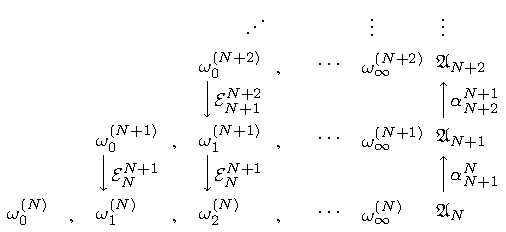
\includegraphics{figure0.pdf}
%\begin{tikzpicture}
%	
%	\draw (0.25,0.25) node[right]{$\omega^{(N)}_{0}$} (1.75,0.25) node[right]{$\omega^{(N)}_{1}$} (3.5,0.25) node[right]{$\omega^{(N)}_{2}$}
%	(5.5,0.25) node[right]{$\dots$} (6.25,0.25) node[right]{$\omega^{(N)}_\infty$} (7.5,0.25) node[right]{$\mathfrak{A}_N$};
%	%\draw[->] (1.2,0.25) to (1.7,0.25);
%	\draw (1.45,0.25) node[below]{,};
%	%\draw[->] (2.95,0.25) to (3.45,0.25);
%	\draw (3.2,0.25) node[below]{,};
%	%\draw[->] (4.7,0.25) to (5.2,0.25);
%	\draw (4.95,0.25) node[below]{,};
%	
%	\draw (1.75,1.5) node[right]{$\omega^{(N+1)}_{0}$} (3.5,1.5) node[right]{$\omega^{(N+1)}_{1}$} (5.5,1.5)
%	node[right]{$\dots$} (6.25,1.5) node[right]{$\omega^{(N+1)}_\infty$}  (7.5,1.5) node[right]{$\mathfrak{A}_{N+1}$};
%	%\draw[->] (2.95,1.5) to (3.45,1.5);
%	\draw (3.2,1.5) node[below]{,};
%	%\draw[->] (4.7,1.5) to (5.2,1.5);
%	\draw (4.95,1.5) node[below]{,};
%	
%	\draw (2,0.875) node[right]{$\mathcal{E}^{N+1}_{N}$} (3.75,0.875) node[right]{$\mathcal{E}^{N+1}_{N}$};
%	\draw[->] (2,1.2) to (2,0.6);
%	\draw[->] (3.75,1.2) to (3.75,0.6);
%	\draw[<-] (7.75,1.2) to (7.75,0.6); 
%	\draw (7.75,0.875) node[right]{$\alpha^{N}_{N+1}$};
%	
%	\draw (3.5,2.75) node[right]{$\omega^{(N+2)}_{0}$} (5.5,2.75)
%	node[right]{$\dots$} (6.25,2.75) node[right]{$\omega^{(N+2)}_\infty$} (7.5,2.75) node[right]{$\mathfrak{A}_{N+2}$};
%	%\draw[->] (4.7,2.75) to (5.2,2.75);
%	\draw (4.95,2.75) node[below]{,};
%	
%	\draw (3.75,2.125) node[right]{$\mathcal{E}^{N+2}_{N+1}$};
%	\draw[->] (3.75,2.45) to (3.75,1.85);
%	\draw[<-] (7.75,2.45) to (7.75,1.85);
%	\draw (7.75,2.125) node[right]{$\alpha^{N+1}_{N+2}$};
%	
%	\node[right] at (4.25,3.475) {$\iddots$};
%	\node[right] at (6.375,3.475) {$\vdots$};
%	\node[right] at (7.575,3.475) {$\vdots$};
%\end{tikzpicture}
\caption{Wilson's triangle of renormalization \cite{wilsonRenormalizationGroupCritical1975, stottmeisterOperatoralgebraicRenormalizationWavelets2020}: Vertical lines represent renormalization steps, either by coarse graining states ($\cE$'s) or by refining fields ($\alpha$'s). Horizontal lines represent sequences of renormalized states at a fixed scale.}
\label{fig:statetrianglerg}
\end{center}
\end{figure}

The \emph{renormalization group} is the collection $\{\alpha^{N_{1}}_{N_{2}}\}_{N_{2}>N_{1}}$, satisfying $\alpha^{N_{2}}_{N_{3}}\circ\alpha^{N_{1}}_{N_{2}}\!=\!\alpha^{N_{1}}_{N_{3}}$.
A \textit{scaling limit} $\rho^{(N)}_{\infty}$ is a limit state $\lim_{M\rightarrow\infty}\rho^{(N)}_{M}\!=\!\rho^{(N)}_{\infty}$ on $\fA_N$, which is stable under coarse-graining \footnote{Note that we have described everything in terms of trace-class density operators, however, the considerations here may be extended directly to states on $C^*$ algebras without a density-operator representation. See \cite{osborneConformal2021} for further information.}:
\begin{align}
\label{eq:staterglimit}
\mathcal{E}_{N_1}^{N_2}(\rho^{(N_{2})}_{\infty}) & \!=\!\rho^{(N_{1})}_{\infty}.
\end{align}
Finding a limit state usually requires a scale-dependent redefinition of bare coupling constants according to \emph{renormalization conditions}.
Ultimately, we are interested in the \emph{double scaling limit} $\rho_{\infty}^{(\infty)}\!\equiv\!\lim_{N\rightarrow \infty} \rho_\infty^{(N)}$, realising the continuum limit, see Fig.~\ref{fig:statetrianglerg} (existing because of \eqref{eq:staterglimit} without additional constraints). The scaling limit of the family of Hamiltonians $H^{(N)}_{0}$ is understood via a limit, $\tau^{(\infty)}_{t}$, of discretised Heisenberg dynamics $\tau^{(N)}_{t}\!=\!e^{i t H^{(N)}_{0}}\!(\!\ \cdot\!\ )e^{-i t H^{(N)}_{0}}$. Thus, a triple $\{\fA,\rho,\tau_{t}\}$, where $\fA\!\equiv\! \fA_{\infty}$, $\rho\!\equiv\!\rho^{(\infty)}_{\infty}$, and $\tau_t\!\equiv\! \tau_t^{(\infty)}$, is called a \emph{scaling limit} of $\{\fA_{N},\cH_{N},H^{(N)}_{0}\}_{N}$.

The success of OAR depends crucially on the coarse-graining map $\mathcal{E}$, chosen to preserve the quantum coherence in low-energy degrees of freedom. Two particularly powerful procedures are realised in real and momentum space. For the real-space scheme we choose 
\begin{align}
\label{eq:waveletrg}
	\alpha_{N+1}^N(\psi_x^{(j)}) & \!=\!\sum_{l\in \mathbb{Z}} c_l \psi_{x-\vep_{N+1}l}^{(j)},
\end{align}
for the \emph{low-pass filter} $\{c_l\}_{l\in \mathbb{Z}}$ of a compactly supported orthogonal scaling function $s(x)\!=\!\sqrt{2}\!\sum_{l\in\mathbb{Z}} \!c_l s(2x\!-\!l)$ \footnote{Only finitely many of the $c_l$ are nonzero, so that the sum appearing in (\ref{eq:waveletrg}) is well defined as long as $N$  is larger than the number of nonzero terms.}.
%\begin{align*}
%	s(x) & \!=\!\sqrt{2} \sum_{l\in\mathbb{Z}}  c_l s(2x -l).
%\end{align*}
Daubechies's D4 wavelet \cite{daubechiesTenLecturesWavelets1992} furnishes an explicit example with coefficients $c_0\!=\!\frac{1}{4\sqrt{2}}(1\!+\!\sqrt{3})$, $c_1\!=\!\frac{1}{4\sqrt{2}}(3\!+\!\sqrt{3})$, $c_2\!=\!\frac{1}{4\sqrt{2}}(3\!-\!\sqrt{3})$, and $c_3\!=\!\frac{1}{4\sqrt{2}}(1\!-\!\sqrt{3})$. However, the simulation of observables with unbounded continuum limit can necessitate wavelets of higher regularity.
Renormalized fermion operators, $\widetilde{\psi}_x^{(j)}\!\equiv\!\alpha_{N+1}^N(\psi_x^{(j)})$, act on the fine-grained lattice, with lattice spacing $\frac12\vep$. Fig.~\ref{fig:oar} illustrates the resulting real-space OAR.

\begin{figure}[h]
	\begin{center}
	\scalebox{0.9}{
	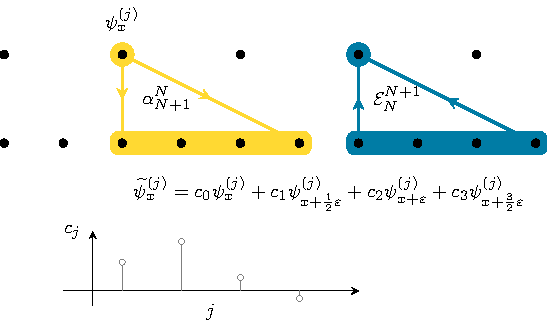
\includegraphics{figure1.pdf}
%		\begin{tikzpicture}
%			\begin{scope}[very thick,decoration={markings, mark=at position 0.5 with {\arrow{stealth}}}] 
%		  	\draw[postaction={decorate}, color=banana] (2,1.5) -- (2,0);
%				\draw[postaction={decorate}, color=banana] (2,1.5) -- (5,0);
%		  	\draw[postaction={decorate}, color=cgblue] (6,0) -- (6,1.5);
%				\draw[postaction={decorate}, color=cgblue] (9,0) -- (6,1.5);		
%			\end{scope}
%			\def\x{0.2};
%			\def\y{2.5};
%%			\draw[stealth-stealth] (12,2+2*\x) -- (14,2+2*\x);
%%			\draw (12,2+\x) -- (12,2+3*\x);
%%			\draw (14,2+\x) -- (14,2+3*\x);
%%			\draw (13,2+3*\x) node {$\vep$};
%%			\draw[stealth-stealth] (12,2*\x) -- (13,2*\x);
%%			\draw (12,\x) -- (12,3*\x);
%%			\draw (13,\x) -- (13,3*\x);
%%			\draw (12.5,3.5*\x) node {$\frac{\vep}{2}$};
%			\draw (2.75,0.75) node {$\alpha^{N}_{N+1}$};
%			\draw (6.65,0.75) node {$\mathcal{E}^{N+1}_{N}$};
%			\draw (2,1.5+3*\x) node {$\psi_x^{(j)}$};
%			\draw[rounded corners, draw=none, fill=banana] (2-\x, -\x) rectangle (5+\x, \x) {};
%			\draw[draw=none, fill=banana] (2,1.5) circle (0.2);
%			\draw[rounded corners, draw=none, fill=cgblue] (6-\x, -\x) rectangle (9+\x, \x) {};
%			\draw[draw=none, fill=cgblue] (6,1.5) circle (0.2);
%			\foreach \j in {0, 2, ..., 9} {
%				\fill (\j,1.5) circle (2pt);
%			}
%			\foreach \j in {0, 1, ..., 9} {
%				\fill (\j,0) circle (2pt);
%			}
%			\draw[-stealth] (1,-\y) -- (6,-\y); 
%			\draw[-stealth] (1.5,-\y-0.25) -- (1.5,-\y+1); 
%			\draw[color=gray] (2,-\y) -- (2,0.4830-\y);
%			\draw[color=gray,fill=white] (2,0.4830-\y) circle (0.05);
%			\draw[color=gray] (3,-\y) -- (3,0.8365-\y);
%			\draw[color=gray,fill=white] (3,0.8365-\y) circle (0.05);
%			\draw[color=gray] (4,-\y) -- (4,0.2241-\y);
%			\draw[color=gray,fill=white] (4,0.2241-\y) circle (0.05);
%			\draw[color=gray] (5,-\y) -- (5,-0.1294-\y);
%			\draw[color=gray,fill=white] (5,-0.1294-\y) circle (0.05);
%		%	\draw[color=gray] (2,0.4830-\y) -- (3,0.8365-\y) -- (4,0.2241-\y) -- (5,-0.1294-\y);
%			\draw (3.5,-0.35-\y) node {$j$};
%			\draw (1.15,1-\y) node {$c_j$};
%			\draw (5.5,-0.85) node {$\widetilde{\psi}_{x}^{(j)}=c_0 \psi_{x}^{(j)} + c_1 \psi_{x+\frac{1}{2}\vep}^{(j)} + c_2 \psi_{x+\vep}^{(j)} + c_3 \psi_{x+\frac{3}{2}\vep}^{(j)}$};
%		\end{tikzpicture}
		}
	\caption{Operator algebraic renormalization in real space for the wavelet D$4$. $\alpha^{N}_{N+1}$ and $\mathcal{E}^{N+1}_{N}$ denote the RG maps in the Heisenberg (respectively, Schr\"odinger) picture, and $c_j$ is the associated low-pass filter.}\label{fig:oar}
	\end{center}
\end{figure}

The momentum-space RG maps are defined on the Fourier-transformed operators, $\widehat{\psi}_k^{(j)}\!\equiv\!\sum_{x\in\Lambda_N} e^{-ikx}\psi_x^{(j)}$, 
by only retaining those associated to long wavelengths up to a momentum cutoff $|k|\!\le\! \frac{\pi L_{M}}{L}$, with short wavelength degrees of freedom $|k|\!>\!\frac{\pi L_{M}}{L}$ traced out,
\begin{align*}
	\alpha_N^M(\widehat{\psi}_k^{(j)}) &\!=\!2^{\frac12(N-M)} \chi_M(k) \widehat{\psi}_k^{(j)},
\end{align*}
where $\chi_M(k)\!=\!1$ if $k\in \frac{\pi}{L}\{-L_{M}+\tfrac12,..., L_{M}+\tfrac12\}$ and $0$ otherwise.
Both RG maps $\alpha_N^M$, in real and momentum space, satisfy the composition rules $\alpha^{N_{2}}_{N_{3}}\circ\alpha^{N_{1}}_{N_{2}}\!=\!\alpha^{N_{1}}_{N_{3}}$.

\paragraph*{Discretised Virasoro generators.} With the basic kinematical and dynamical data in hand we turn to the quantum simulation of conformal symmetries and its associated \emph{Virasoro algebra} of generators spanned by $L_k$, $k\in\frac{\pi}{L}\mathbb{Z}$ and the \emph{central charge} $c$, satisfying 
\begin{align*}
	[L_k,L_l] &\!=\!\tfrac{L}{\pi}(k\!-\!l)L_{k+l}\!+\!\frac{c}{12}((\tfrac{L}{\pi}k)^3\!-\!(\tfrac{L}{\pi}k))\delta_{k+l,0}.
\end{align*}
Several of the generators are directly related to more familiar observables, for example, the CFT Hamiltonian, $H^{\text{CFT}}\!=\!\tfrac{\pi}{L}\left(L_0\!+\!\overline{L}_0\!-\!\tfrac{c}{12}\right)$, and total momentum, $P^{\text{CFT}} \!=\!\tfrac{\pi}{L}\left(L_0\!-\!\overline{L}_0\right)$.
%\begin{align*}
%	H^{\text{CFT}} &\!=\!\tfrac{\pi}{L}\left(L_0\!+\!\overline{L}_0\!-\!\tfrac{c}{12}\right), & P^{\text{CFT}} &\!=\!\tfrac{\pi}{L}\left(L_0\!-\!\overline{L}_0\right).
%\end{align*}
To approximate $L_k$ on a lattice at scale $N$ we exploit an insightful ansatz due to Koo and Saleur \cite{kooRepresentationsVirasoroAlgebra1994b}; we begin by introducing the Fourier modes of the lattice Hamiltonian density\footnote{For massless Dirac fermions: $h_x^{(N)}\!=\!\tfrac{1}{\vep_N^2}\big(\psi^{(1)\!\ \dag}_{x+\varepsilon_{N}}\psi^{(2)}_{x}\!-\!\psi^{(1)\!\ \dag}_{x}\psi^{(2)}_{x}\!+\!\psi^{(2)\!\ \dag}_{x-\varepsilon_{N}}\psi^{(1)}_{x}\!-\!\psi^{(2)\!\ \dag}_{x}\psi^{(1)}_{x}\!+\!\textup{h.c.}\big)$.} (symmetric around $x$ to obtain the correct scaling limit):
\begin{align*}
	H_k^{(N)} \!\!\equiv\! \vep_N \tfrac{L}{\pi} \sum_{x} e^{ikx} h_x^{(N)},
\end{align*} 
and then defining 
\begin{align}
\label{eq:koosaleur}
	L_k^{(N)} & \!\!=\!\tfrac{1}{2}\Big(\!H_k^{(N)}\!\!+\!\tfrac{\pi\frac{1}{2}\vep_N}{L \sin(\frac{1}{2}\vep_N k)}[H_k^{(N)}\!,\!H_0^{(N)}]\Big)\;,
	%\!+\!\tfrac{c}{24}\delta_{k,0},
\end{align}
with an analogous formula for $\overline{L}_k^{(N)}$. The ansatz (\ref{eq:koosaleur}) leads to realisations of CFTs with $c\!=\!0$, $c\!=\!\tfrac{1}{2}$, and $c\!=\!1$ depending on the choice of representation. For $c\!=\!0$, we use the defining representation of the CAR algebra corresponding to the ground state associated with a vanishing stress-energy tensor. Central charges $c\!=\!1$ or $\tfrac{1}{2}$ arise in the representation of either a complex or a real chiral component, the latter via a projection on positive (or negative) momenta, associated with the ground state of the massless free fermion Hamiltonian \cite{osborneConformal2021}.

The crucial observation underlying our quantum simulation algorithm is that $L_k^{(N)}$ so defined in (\ref{eq:koosaleur}) are sums of densities. Therefore, we may employ standard quantum algorithms targeting the dynamics of local Hamiltonians to simulate their exponentials \footnote{We actually simulate hermitian linear combinations of $L_k^{(N)}$ and $\overline{L}_k^{(N)}$ to ensure unitary dynamics.}; since the behaviour of these methods is well understood we focus on new challenges arising in the continuum limit.

\paragraph*{Preparing the initial state.} We initialise the $2n$ qubits of the quantum computer into a discrete approximation of the desired state; for the ground state $|\Omega\rangle$ of the scaling limit we use  $|\Omega_N\rangle$; states in the conformal blocks are found by applying Virasoro generators to $|\Omega\rangle$. (Although our algorithm works for any quantum states with a sensible scaling limit.) Here, we employ a particularly parsimonious quantum circuit to prepare $|\Omega_N\rangle$ adapted from \cite{verstraeteQuantumCircuitsStrongly2009} (see Fig.~\ref{fig:fft}): the quantum spin Hamiltonian (\ref{eq:qsham}) may be diagonalized, $H_0^{(N)}\!=\!U_{\text{FT}}U_{\text{B}} D^{(N)}_0 U_{\text{B}}^\dag U_{\text{FT}}^\dag$, by a quantum circuit for a (fast) fourier transform $U_{\text{FT}}$ followed by a Bogoliubov transformation $U_{\text{B}}$, where $D^{(N)}_0$ is diagonal. This  realises the ground state from a product state:
\begin{align*}
	|\Omega_N\rangle & \!=\!U_{\text{FT}}U_{\text{B}} \bigotimes_{k\in \Gamma_{N+1}} |\!\leftarrow\rangle.
\end{align*}
With the qubit registers in the discrete approximation of the ground state we apply the desired generators $A$ and $B$ for the correlation function to $|\Omega_N\rangle$. For concreteness we focus on the momentum-space RG.
\begin{widetext}

\begin{figure}[h]
	\begin{center}
	\scalebox{0.9}{
		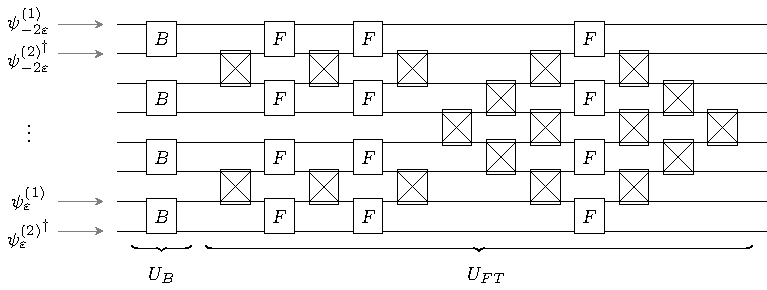
\includegraphics{figure2.pdf}
%		\begin{tikzpicture}
%			\def\x{0.05};
%			\def\y{2.5};
%			\draw (-2,3.5+\x) node {$\psi^{(1)}_{-2\vep}$};
%			\draw[color=gray,-stealth] (-1.5, 3.5) -- (-0.75, 3.5); 
%			\draw (-2,3-\x) node {${\psi^{(2)}_{-2\vep}}^{\!\!\!\dag}$};
%			\draw[color=gray,-stealth] (-1.5, 3) -- (-0.75, 3); 
%			\draw (-2,0.5+\x) node {$\psi^{(1)}_{\vep}$};
%			\draw[color=gray,-stealth] (-1.5, 0.5) -- (-0.75, 0.5); 
%			\draw (-2,0-\x) node {${\psi^{(2)}_{\vep}}^\dag$};
%			\draw[color=gray,-stealth] (-1.5, 0) -- (-0.75, 0); 
%			\draw (-2,1.75) node {$\vdots$};
%			\foreach \j in {0, 0.5, ..., 3.5} {
%				\draw (-0.5,\j) -- (10.5,\j);
%			}
%			\foreach \j in {0, 1, ..., 3.5} {
%				\draw[fill = white] (0,\j-\x) rectangle (0.5, \j+0.5+\x);
%				\draw (0.25, \j+0.25) node {$B$};
%			}
%			\foreach \j in {0.5,2.5} {
%				\draw[fill = white] (1.25,\j-\x) rectangle (1.75, \j+0.5+\x);
%				\draw (1.25,\j) -- (1.75,\j);
%				\draw (1.25,\j+0.5) -- (1.75,\j+0.5);
%				\draw (1.25,\j) -- (1.75,\j+0.5);
%				\draw (1.25,\j+0.5) -- (1.75,\j);				
%			}
%			\foreach \j in {0, 1, ..., 3.5} {
%				\draw[fill = white] (2,\j-\x) rectangle (2.5, \j+0.5+\x);
%				\draw (2.25, \j+0.25) node {$F$};
%			}
%			\foreach \j in {0.5,2.5} {
%				\draw[fill = white] (2.75,\j-\x) rectangle (3.25, \j+0.5+\x);
%				\draw (2.75,\j) -- (3.25,\j);
%				\draw (2.75,\j+0.5) -- (3.25,\j+0.5);
%				\draw (2.75,\j) -- (3.25,\j+0.5);
%				\draw (2.75,\j+0.5) -- (3.25,\j);				
%			}
%			\foreach \j in {0, 1, ..., 3.5} {
%				\draw[fill = white] (3.5,\j-\x) rectangle (4, \j+0.5+\x);
%				\draw (3.75, \j+0.25) node {$F$};
%			}
%			\foreach \j in {0.5,2.5} {
%				\draw[fill = white] (4.25,\j-\x) rectangle (4.75, \j+0.5+\x);
%				\draw (4.25,\j) -- (4.75,\j);
%				\draw (4.25,\j+0.5) -- (4.75,\j+0.5);
%				\draw (4.25,\j) -- (4.75,\j+0.5);
%				\draw (4.25,\j+0.5) -- (4.75,\j);				
%			}
%			\foreach \j in {1.5} {
%				\draw[fill = white] (5,\j-\x) rectangle (5.5, \j+0.5+\x);
%				\draw (5,\j) -- (5.5,\j);
%				\draw (5,\j+0.5) -- (5.5,\j+0.5);
%				\draw (5,\j) -- (5.5,\j+0.5);
%				\draw (5,\j+0.5) -- (5.5,\j);	
%			}
%			\foreach \j in {1, 2} {
%				\draw[fill = white] (5.75,\j-\x) rectangle (6.25, \j+0.5+\x);
%				\draw (5.75,\j) -- (6.25,\j);
%				\draw (5.75,\j+0.5) -- (6.25,\j+0.5);
%				\draw (5.75,\j) -- (6.25,\j+0.5);
%				\draw (5.75,\j+0.5) -- (6.25,\j);	
%			}
%			\foreach \j in {0.5, 1.5, 2.5} {
%				\draw[fill = white] (6.5,\j-\x) rectangle (7, \j+0.5+\x);
%				\draw (6.5,\j) -- (7,\j);
%				\draw (6.5,\j+0.5) -- (7,\j+0.5);
%				\draw (6.5,\j) -- (7,\j+0.5);
%				\draw (6.5,\j+0.5) -- (7,\j);	
%			}
%			\foreach \j in {0, 1, ..., 3.5} {
%				\draw[fill = white] (7.25,\j-\x) rectangle (7.75, \j+0.5+\x);
%				\draw (7.5, \j+0.25) node {$F$};
%			}
%			\foreach \j in {0.5, 1.5, 2.5} {
%				\draw[fill = white] (8,\j-\x) rectangle (8.5, \j+0.5+\x);
%				\draw (8,\j) -- (8.5,\j);
%				\draw (8,\j+0.5) -- (8.5,\j+0.5);
%				\draw (8,\j) -- (8.5,\j+0.5);
%				\draw (8,\j+0.5) -- (8.5,\j);	
%			}
%			\foreach \j in {1, 2} {
%				\draw[fill = white] (8.75,\j-\x) rectangle (9.25, \j+0.5+\x);
%				\draw (8.75,\j) -- (9.25,\j);
%				\draw (8.75,\j+0.5) -- (9.25,\j+0.5);
%				\draw (8.75,\j) -- (9.25,\j+0.5);
%				\draw (8.75,\j+0.5) -- (9.25,\j);	
%			}
%			\foreach \j in {1.5} {
%				\draw[fill = white] (9.5,\j-\x) rectangle (10, \j+0.5+\x);
%				\draw (9.5,\j) -- (10,\j);
%				\draw (9.5,\j+0.5) -- (10,\j+0.5);
%				\draw (9.5,\j) -- (10,\j+0.5);
%				\draw (9.5,\j+0.5) -- (10,\j);	
%			}
%			\draw [decorate, decoration = {calligraphic brace}] (0.75,-0.25) --  (-0.25,-0.25);
%			\draw (0.25,-0.75) node {$U_B$};
%			\draw [decorate, decoration = {calligraphic brace}] (10.25,-0.25) --  (1,-0.25);
%			\draw (5.75,-0.75) node {$U_{FT}$};
%		\end{tikzpicture}
	}
	\caption{Illustrating the ground-state preparation circuit for $4$ sites. The fermion operators (left), identified with the corresponding sites in the spin model via the Jordan-Wigner mapping.}\label{fig:fft}
	\end{center}
\end{figure}

\end{widetext}
In the case of correlation functions for operators $\widehat{\psi}_k^{(j)}$, with $|k|\le \frac{\pi L_{M}}{L}$, local in momentum space we have that
\begin{align*}
	\widehat{\psi}_k^{(j)} & \!\!=\!U_{\text{FT}}\sigma^x_{-\frac{\pi}{L}(-\!L_{N\!+\!1}\!+\!\frac12)}...\sigma^x_{k\!-\!\frac{\pi}{L}} \tfrac{1}{2}(\sigma_{k}^z\!-\!(-1)^ji\sigma_{k}^y)U_{\text{FT}}^\dag,
\end{align*}
The action of this nonunitary operator may be simulated, e.g., by introducing an ancilla qubit initialised in the state $\frac{1}{\sqrt{2}}(|0\rangle+|1\rangle\!)$, applying the unitary gate $V\!=\!U_{\text{FT}}\sigma^x_{-\frac{\pi}{L}(-\!L_{N\!+\!1}\!+\!\frac12)}... \sigma^x_{k\!-\!\frac{\pi}{L}}(\sigma_{k}^z\!\otimes\!|0\rangle\langle
0|\!-\!(-1)^ji\sigma_{k}^y\!\otimes\!|1\rangle\langle
1|)U_{\text{FT}}^\dag$ to the momentum-space representation of the ground state $U_{\text{FT}}U_{\text{B}}\bigotimes_{k\in \Gamma_{N+1}} |\!\!\leftarrow\rangle$, and then measuring the $\sigma^x$ operator on the ancilla qubit, postselecting on the positive outcome. Repeating this procedure a constant number of times ensures the correct state is produced with high probability (for a constant number of field operators). In this way we may easily prepare
the initial state $\prod_{k_l}\widehat{\psi}_{k_l}^{(j_l)}|\Omega_N\rangle$. (Applying field operators local in real space is more involved, e.g., using wavelets as above. See \cite{osborneConformal2021} for further details.) The resulting initial state is denoted $|\Phi_{\text{init}}\rangle$.

\paragraph*{Simulating dynamics.} Having prepared the initial state we may apply local conformal transformations. In terms of the Fourier-transformed single-component fermion operators, $\hat{\psi}^{(1)}_{k}\!=\!\tfrac{1}{2}(\hat{a}_{k}\!+\!\hat{a}_{k\!+\!\frac{\pi}{\varepsilon_{N\!+\!1}}})$, $\hat{\psi}^{(2)}_{k}\!=\!\tfrac{1}{2}e^{i\varepsilon_{N\!+\!1}k}(\hat{a}^{\dag}_{-k}\!-\!\hat{a}^{\dag}_{-k\!+\!\frac{\pi}{\varepsilon_{N\!+\!1}}})$, these are generated by hermitian linear combinations of the following Koo-Saleur operators:

\begin{widetext}
\begin{align}
	L_k^{(N)} & = \tfrac{1}{8\pi}e^{-\frac{i}{4}\varepsilon_{N}k}\sum_{l,l'\in\Gamma_{N+1}} \!\!\! \begin{pmatrix}
		\hat{a}_{l'} \\ \hat{a}^{\dag}_{-l'}
	\end{pmatrix}^{\dag}
	\delta_{k,l'-l\!\!\!\!\mod\frac{2\pi}{\varepsilon_{N}}}
	\ell^{(N)}_{k}(l',l) \begin{pmatrix}
		\hat{a}_{l} \\ \hat{a}^{\dag}_{-l}
	\end{pmatrix}\;, \\ \nonumber
	\ell^{(N)}_{k}(l',l) & = \tfrac{1}{2}\!\begin{pmatrix} \hspace{-0cm} -e^{\frac{i}{4}\varepsilon_{N}k}\sin(\varepsilon_{N}(l+\tfrac{k}{2})\!) & \hspace{-0cm} -i(e^{\frac{i}{4}\varepsilon_{N}k}\sin(\varepsilon_{N}\tfrac{l}{2})+e^{-\frac{i}{4}\varepsilon_{N}k}\sin(\varepsilon_{N}\tfrac{l+k}{2})\!) \\ i(e^{\frac{i}{4}\varepsilon_{N}k}\sin(\varepsilon_{N}\tfrac{l'-k}{2})+e^{-\frac{i}{4}\varepsilon_{N}k}\sin(\varepsilon_{N}\tfrac{l'}{2})\!) & -e^{-\frac{i}{4}\varepsilon_{N}k}\sin(\varepsilon_{N}\tfrac{l+l'}{2}) \end{pmatrix}\;.
%	L_k^{(N)} = \frac{1}{4\pi}\sum_{l\in\Gamma_{N+1}} \begin{pmatrix}
%		\widehat{\psi}^{(1)}_{l+2k} & \widehat{\psi}^{(2)}_{l+2k}
%	\end{pmatrix} \begin{pmatrix}
%		0 & e^{-i\varepsilon_{N+1}(l+2k)}-1 \\ e^{i\varepsilon_{N+1}l}-1 & -2\sin(\varepsilon_{N+1}(l+k))
%	\end{pmatrix} \begin{pmatrix}
%		\widehat{\psi}^{(1)}_{l} \\ \widehat{\psi}^{(2)}_{l}.
%	\end{pmatrix}
\end{align}
\end{widetext}

These generators are $(2k\!+\!1)$-local in the momentum representation and may be simulated via a Suzuki-Trotter decomposition. (A state-of-the-art implementation will make use of the optimal simulation algorithms.)
Applying the generator puts the quantum register in the state
\begin{align*}
	|\Phi'\rangle & \!=\! e^{-i s (L_k^{(N)}+\overline{L}_k^{(N)})}|\Phi_{\text{init}}\rangle\;.
\end{align*}
The $k\!=\!0$ case reduces to simulating the unitary Hamiltonian evolution.

\paragraph*{Measuring observables.} To measure a desired observable $\widehat{O}$, e.g., $\widehat{O}\!=\!\widehat{\psi}_k^{(j)}$, one may employ standard phase estimation \cite{nielsenQuantumComputationQuantum2000,childsQuantumSearchMeasurement2002}. This requires the addition of $r$ ancilla qubits to represent the readout, where $r$ is the required to be large enough to resolve all of the eigenvalues of $\widehat{O}$. Repeating this procedure delivers an estimate for the expectation value
\begin{align*}
	\langle\widehat{O} \rangle & \!=\! \langle\Phi'|\widehat{O}|\Phi'\rangle\;.
\end{align*}

\paragraph*{Error analysis.} The errors in the quantum simulation arise from several sources. The first, and easiest to control, is the quantum projection noise arising the estimation of $\langle \widehat{O}\rangle$. This may be reduced in the standard way via parallel repetition. The second salient source of error arises from the quantum simulation of the unitary $e^{-i s (L_k^{(N)}+\overline{L}_k^{(N)})}$ via, e.g., product formulas \cite{childsNearlyOptimalLattice2019}, and may be reduced by exploiting higher-order approximations. Exploiting state-of-the art estimates, one requires quantum gates $(nt)^{1+o(1)}$ to reduce this error to below $\delta/2$. The state preparation is considered exact (up to the gate compilation required to implement the single- and two-qubit unitaries required). The fourth source of error arises from the discretization itself. This is deeply nontrivial and requires an extensive and challenging analysis, discussed in the companion paper \cite{osborneConformal2021}, which implies the existence, for a given desired accuracy $\delta$ and $t\!\leq\!T$, of a constant size $N(\delta,T)$ lattice achieving this accuracy. The dependence of $N$ on $\delta$ and $T$ is nontrivial, however, numerical experiments --- see the Supplementary Material --- indicate that $N(\delta,T)\!\sim\!C_{T}\delta^{-2}$ (computing dynamical correlation functions involving Virasoro generators), e.g., a D$10$ wavelet can achieve an accuracy of $\delta\!=\!1/2$ on a lattice of $128$ sites (see Supplementary Material).

\paragraph*{Extensions.} The presented algorithm generalises to the approximation of lattice currents of Wess-Zumino-Witten models, which we can simulate using $D$ copies of the realisation exploited above \cite{osborneConformal2021}. The Ising CFT may also be directly targeted using a modified approach. 

\paragraph*{Conclusions and future directions.} We have demonstrated that quantum computers may be exploited to simulate the local conformal dynamics of CFTs. The simulation algorithms are built invoking operator-algebraic renormalization realising the continuum limit as a sequence of lattice models. Local conformal transformations are simulated via the Koo-Saleur generators. Generalizations to the Ising CFT and WZW models are directly possible \cite{osborneConformal2021}.

\begin{acknowledgments}
The authors would like to thank R.\ F.\ Werner for valuable discussions about inductive limits in quantum theory. AS would like to thank Y.\ Tanimoto for helpful discussions concerning the essential self-adjointness of smeared Virasoro generators. This work was supported, in part, by the DFG through SFB 1227 (DQ-mat), Quantum Valley Lower Saxony, and funded by the Deutsche Forschungsgemeinschaft (DFG, German Research Foundation) under Germanys Excellence Strategy EXC-2123 QuantumFrontiers 390837967. 
\end{acknowledgments}

\begin{thebibliography}{61}%
\makeatletter
\providecommand \@ifxundefined [1]{%
 \@ifx{#1\undefined}
}%
\providecommand \@ifnum [1]{%
 \ifnum #1\expandafter \@firstoftwo
 \else \expandafter \@secondoftwo
 \fi
}%
\providecommand \@ifx [1]{%
 \ifx #1\expandafter \@firstoftwo
 \else \expandafter \@secondoftwo
 \fi
}%
\providecommand \natexlab [1]{#1}%
\providecommand \enquote  [1]{``#1''}%
\providecommand \bibnamefont  [1]{#1}%
\providecommand \bibfnamefont [1]{#1}%
\providecommand \citenamefont [1]{#1}%
\providecommand \href@noop [0]{\@secondoftwo}%
\providecommand \href [0]{\begingroup \@sanitize@url \@href}%
\providecommand \@href[1]{\@@startlink{#1}\@@href}%
\providecommand \@@href[1]{\endgroup#1\@@endlink}%
\providecommand \@sanitize@url [0]{\catcode `\\12\catcode `\$12\catcode
  `\&12\catcode `\#12\catcode `\^12\catcode `\_12\catcode `\%12\relax}%
\providecommand \@@startlink[1]{}%
\providecommand \@@endlink[0]{}%
\providecommand \url  [0]{\begingroup\@sanitize@url \@url }%
\providecommand \@url [1]{\endgroup\@href {#1}{\urlprefix }}%
\providecommand \urlprefix  [0]{URL }%
\providecommand \Eprint [0]{\href }%
\providecommand \doibase [0]{https://doi.org/}%
\providecommand \selectlanguage [0]{\@gobble}%
\providecommand \bibinfo  [0]{\@secondoftwo}%
\providecommand \bibfield  [0]{\@secondoftwo}%
\providecommand \translation [1]{[#1]}%
\providecommand \BibitemOpen [0]{}%
\providecommand \bibitemStop [0]{}%
\providecommand \bibitemNoStop [0]{.\EOS\space}%
\providecommand \EOS [0]{\spacefactor3000\relax}%
\providecommand \BibitemShut  [1]{\csname bibitem#1\endcsname}%
\let\auto@bib@innerbib\@empty
%</preamble>
\bibitem [{\citenamefont {Douglas}(2012)}]{douglasFoundationsQuantumField2012}%
  \BibitemOpen
  \bibfield  {author} {\bibinfo {author} {\bibfnamefont {M.~R.}\ \bibnamefont
  {Douglas}},\ }\bibfield  {title} {\bibinfo {title} {Foundations of {{Quantum
  Field Theory}}},\ }in\ \href@noop {} {\emph {\bibinfo {booktitle}
  {Proceedings of {{Symposia}} in {{Pure Mathematics}}}}},\ Vol.~\bibinfo
  {volume} {85}\ (\bibinfo  {publisher} {{American Mathematical Society}},\
  \bibinfo {address} {{University of Pennsylvania, Philadelphia, PA}},\
  \bibinfo {year} {2012})\ pp.\ \bibinfo {pages} {105--124}\BibitemShut
  {NoStop}%
\bibitem [{\citenamefont {Seiberg}(2014)}]{seibergNathanSeiberg20152014}%
  \BibitemOpen
  \bibfield  {author} {\bibinfo {author} {\bibfnamefont {N.}~\bibnamefont
  {Seiberg}},\ }\href@noop {} {\bibinfo {title} {2015 {{Breakthrough Prize}} in
  {{Fundamental Physics Symposium}} - {{YouTube}}}},\ \bibinfo {howpublished}
  {https://www.youtube.com/watch?v=Hi3e0HVxlFo} (\bibinfo {year}
  {2014})\BibitemShut {NoStop}%
\bibitem [{\citenamefont {Witten}(2018)}]{wittenAPSMedalExceptional2018}%
  \BibitemOpen
  \bibfield  {author} {\bibinfo {author} {\bibfnamefont {E.}~\bibnamefont
  {Witten}},\ }\bibfield  {title} {\bibinfo {title} {{{APS Medal}} for
  {{Exceptional Achievement}} in {{Research}}: {{Invited}} article on
  entanglement properties of quantum field theory},\ }\href@noop {} {\bibfield
  {journal} {\bibinfo  {journal} {Rev. Modern Phys.}\ }\textbf {\bibinfo
  {volume} {90}},\ \bibinfo {pages} {045003} (\bibinfo {year}
  {2018})}\BibitemShut {NoStop}%
\bibitem [{\citenamefont
  {Feynman}(1981)}]{feynmanSimulatingPhysicsComputers1981}%
  \BibitemOpen
  \bibfield  {author} {\bibinfo {author} {\bibfnamefont {R.~P.}\ \bibnamefont
  {Feynman}},\ }\bibfield  {title} {\bibinfo {title} {Simulating physics with
  computers},\ }\href@noop {} {\bibfield  {journal} {\bibinfo  {journal} {Int.
  J. Theor. Phys.}\ }\textbf {\bibinfo {volume} {21}},\ \bibinfo {pages} {467}
  (\bibinfo {year} {1981})}\BibitemShut {NoStop}%
\bibitem [{\citenamefont {Lloyd}(1996)}]{lloydUniversalQuantumSimulators1996}%
  \BibitemOpen
  \bibfield  {author} {\bibinfo {author} {\bibfnamefont {S.}~\bibnamefont
  {Lloyd}},\ }\bibfield  {title} {\bibinfo {title} {Universal {{Quantum
  Simulators}}},\ }\href@noop {} {\bibfield  {journal} {\bibinfo  {journal}
  {Science}\ }\textbf {\bibinfo {volume} {273}},\ \bibinfo {pages} {1073}
  (\bibinfo {year} {1996})}\BibitemShut {NoStop}%
\bibitem [{\citenamefont {Abrams}\ and\ \citenamefont
  {Lloyd}(1997)}]{abramsSimulationManyBodyFermi1997a}%
  \BibitemOpen
  \bibfield  {author} {\bibinfo {author} {\bibfnamefont {D.~S.}\ \bibnamefont
  {Abrams}}\ and\ \bibinfo {author} {\bibfnamefont {S.}~\bibnamefont {Lloyd}},\
  }\bibfield  {title} {\bibinfo {title} {Simulation of {{Many}}-{{Body Fermi
  Systems}} on a {{Universal Quantum Computer}}},\ }\href@noop {} {\bibfield
  {journal} {\bibinfo  {journal} {Phys. Rev. Lett.}\ }\textbf {\bibinfo
  {volume} {79}},\ \bibinfo {pages} {2586} (\bibinfo {year}
  {1997})}\BibitemShut {NoStop}%
\bibitem [{\citenamefont {Zalka}(1998)}]{zalkaSimulatingQuantumSystems1998}%
  \BibitemOpen
  \bibfield  {author} {\bibinfo {author} {\bibfnamefont {C.}~\bibnamefont
  {Zalka}},\ }\bibfield  {title} {\bibinfo {title} {Simulating quantum systems
  on a quantum computer},\ }\href@noop {} {\bibfield  {journal} {\bibinfo
  {journal} {Proc. Roy. Soc. of London Ser. A}\ }\textbf {\bibinfo {volume}
  {454}},\ \bibinfo {pages} {313} (\bibinfo {year} {1998})}\BibitemShut
  {NoStop}%
\bibitem [{\citenamefont {Smith}\ \emph {et~al.}(2019)\citenamefont {Smith},
  \citenamefont {Kim}, \citenamefont {Pollmann},\ and\ \citenamefont
  {Knolle}}]{smithSimulatingQuantumManybody2019}%
  \BibitemOpen
  \bibfield  {author} {\bibinfo {author} {\bibfnamefont {A.}~\bibnamefont
  {Smith}}, \bibinfo {author} {\bibfnamefont {M.~S.}\ \bibnamefont {Kim}},
  \bibinfo {author} {\bibfnamefont {F.}~\bibnamefont {Pollmann}},\ and\
  \bibinfo {author} {\bibfnamefont {J.}~\bibnamefont {Knolle}},\ }\bibfield
  {title} {\bibinfo {title} {Simulating quantum many-body dynamics on a current
  digital quantum computer},\ }\href@noop {} {\bibfield  {journal} {\bibinfo
  {journal} {npj Quantum Information}\ }\textbf {\bibinfo {volume} {5}},\
  \bibinfo {pages} {1} (\bibinfo {year} {2019})}\BibitemShut {NoStop}%
\bibitem [{\citenamefont {Zhang}\ \emph {et~al.}(2017)\citenamefont {Zhang},
  \citenamefont {Pagano}, \citenamefont {Hess}, \citenamefont {Kyprianidis},
  \citenamefont {Becker}, \citenamefont {Kaplan}, \citenamefont {Gorshkov},
  \citenamefont {Gong},\ and\ \citenamefont
  {Monroe}}]{zhangObservationManybodyDynamical2017}%
  \BibitemOpen
  \bibfield  {author} {\bibinfo {author} {\bibfnamefont {J.}~\bibnamefont
  {Zhang}}, \bibinfo {author} {\bibfnamefont {G.}~\bibnamefont {Pagano}},
  \bibinfo {author} {\bibfnamefont {P.~W.}\ \bibnamefont {Hess}}, \bibinfo
  {author} {\bibfnamefont {A.}~\bibnamefont {Kyprianidis}}, \bibinfo {author}
  {\bibfnamefont {P.}~\bibnamefont {Becker}}, \bibinfo {author} {\bibfnamefont
  {H.}~\bibnamefont {Kaplan}}, \bibinfo {author} {\bibfnamefont {A.~V.}\
  \bibnamefont {Gorshkov}}, \bibinfo {author} {\bibfnamefont {Z.-X.}\
  \bibnamefont {Gong}},\ and\ \bibinfo {author} {\bibfnamefont
  {C.}~\bibnamefont {Monroe}},\ }\bibfield  {title} {\bibinfo {title}
  {Observation of a many-body dynamical phase transition with a 53-qubit
  quantum simulator},\ }\href@noop {} {\bibfield  {journal} {\bibinfo
  {journal} {Nature}\ }\textbf {\bibinfo {volume} {551}},\ \bibinfo {pages}
  {601} (\bibinfo {year} {2017})}\BibitemShut {NoStop}%
\bibitem [{\citenamefont {Bernien}\ \emph {et~al.}(2017)\citenamefont
  {Bernien}, \citenamefont {Schwartz}, \citenamefont {Keesling}, \citenamefont
  {Levine}, \citenamefont {Omran}, \citenamefont {Pichler}, \citenamefont
  {Choi}, \citenamefont {Zibrov}, \citenamefont {Endres}, \citenamefont
  {Greiner}, \citenamefont {Vuleti{\'c}},\ and\ \citenamefont
  {Lukin}}]{bernienProbingManybodyDynamics2017}%
  \BibitemOpen
  \bibfield  {author} {\bibinfo {author} {\bibfnamefont {H.}~\bibnamefont
  {Bernien}}, \bibinfo {author} {\bibfnamefont {S.}~\bibnamefont {Schwartz}},
  \bibinfo {author} {\bibfnamefont {A.}~\bibnamefont {Keesling}}, \bibinfo
  {author} {\bibfnamefont {H.}~\bibnamefont {Levine}}, \bibinfo {author}
  {\bibfnamefont {A.}~\bibnamefont {Omran}}, \bibinfo {author} {\bibfnamefont
  {H.}~\bibnamefont {Pichler}}, \bibinfo {author} {\bibfnamefont
  {S.}~\bibnamefont {Choi}}, \bibinfo {author} {\bibfnamefont {A.~S.}\
  \bibnamefont {Zibrov}}, \bibinfo {author} {\bibfnamefont {M.}~\bibnamefont
  {Endres}}, \bibinfo {author} {\bibfnamefont {M.}~\bibnamefont {Greiner}},
  \bibinfo {author} {\bibfnamefont {V.}~\bibnamefont {Vuleti{\'c}}},\ and\
  \bibinfo {author} {\bibfnamefont {M.~D.}\ \bibnamefont {Lukin}},\ }\bibfield
  {title} {\bibinfo {title} {Probing many-body dynamics on a 51-atom quantum
  simulator},\ }\href@noop {} {\bibfield  {journal} {\bibinfo  {journal}
  {Nature}\ }\textbf {\bibinfo {volume} {551}},\ \bibinfo {pages} {579}
  (\bibinfo {year} {2017})}\BibitemShut {NoStop}%
\bibitem [{\citenamefont {Jordan}\ \emph {et~al.}(2012)\citenamefont {Jordan},
  \citenamefont {Lee},\ and\ \citenamefont
  {Preskill}}]{jordanQuantumAlgorithmsQuantum2012}%
  \BibitemOpen
  \bibfield  {author} {\bibinfo {author} {\bibfnamefont {S.~P.}\ \bibnamefont
  {Jordan}}, \bibinfo {author} {\bibfnamefont {K.~S.~M.}\ \bibnamefont {Lee}},\
  and\ \bibinfo {author} {\bibfnamefont {J.}~\bibnamefont {Preskill}},\
  }\bibfield  {title} {\bibinfo {title} {Quantum {{Algorithms}} for {{Quantum
  Field Theories}}},\ }\href@noop {} {\bibfield  {journal} {\bibinfo  {journal}
  {Science}\ }\textbf {\bibinfo {volume} {336}},\ \bibinfo {pages} {1130}
  (\bibinfo {year} {2012})}\BibitemShut {NoStop}%
\bibitem [{\citenamefont {Hamed~Moosavian}\ and\ \citenamefont
  {Jordan}(2018)}]{hamedmoosavianFasterQuantumAlgorithm2018}%
  \BibitemOpen
  \bibfield  {author} {\bibinfo {author} {\bibfnamefont {A.}~\bibnamefont
  {Hamed~Moosavian}}\ and\ \bibinfo {author} {\bibfnamefont {S.}~\bibnamefont
  {Jordan}},\ }\bibfield  {title} {\bibinfo {title} {Faster quantum algorithm
  to simulate fermionic quantum field theory},\ }\href@noop {} {\bibfield
  {journal} {\bibinfo  {journal} {Phys. Rev. A}\ }\textbf {\bibinfo {volume}
  {98}},\ \bibinfo {pages} {012332} (\bibinfo {year} {2018})}\BibitemShut
  {NoStop}%
\bibitem [{\citenamefont {Jordan}\ \emph {et~al.}(2014)\citenamefont {Jordan},
  \citenamefont {Lee},\ and\ \citenamefont
  {Preskill}}]{jordanQuantumAlgorithmsFermionic2014}%
  \BibitemOpen
  \bibfield  {author} {\bibinfo {author} {\bibfnamefont {S.~P.}\ \bibnamefont
  {Jordan}}, \bibinfo {author} {\bibfnamefont {K.~S.~M.}\ \bibnamefont {Lee}},\
  and\ \bibinfo {author} {\bibfnamefont {J.}~\bibnamefont {Preskill}},\
  }\bibfield  {title} {\bibinfo {title} {Quantum {{Algorithms}} for {{Fermionic
  Quantum Field Theories}}}} (\bibinfo {year} {2014}),\ \bibinfo {note}
  {arXiv:1404.7115}\BibitemShut {NoStop}%
\bibitem [{\citenamefont
  {Preskill}(2018)}]{preskillSimulatingQuantumField2018}%
  \BibitemOpen
  \bibfield  {author} {\bibinfo {author} {\bibfnamefont {J.}~\bibnamefont
  {Preskill}},\ }\bibfield  {title} {\bibinfo {title} {{Simulating Quantum
  Field Theory with a Quantum Computer}},\ }in\ \href
  {https://doi.org/10.48550/arXiv.1811.10085} {\emph {\bibinfo {booktitle} {The
  36th Annual International Symposium on Lattice Field Theory - LATTICE2018}}}\
  (\bibinfo {year} {2018})\BibitemShut {NoStop}%
\bibitem [{\citenamefont
  {Wilson}(1975)}]{wilsonRenormalizationGroupCritical1975}%
  \BibitemOpen
  \bibfield  {author} {\bibinfo {author} {\bibfnamefont {K.~G.}\ \bibnamefont
  {Wilson}},\ }\bibfield  {title} {\bibinfo {title} {{The renormalization
  group: Critical phenomena and the Kondo problem}},\ }\href
  {https://doi.org/10.1103/RevModPhys.47.773} {\bibfield  {journal} {\bibinfo
  {journal} {Reviews of Modern Physics}\ }\textbf {\bibinfo {volume} {47}},\
  \bibinfo {pages} {773} (\bibinfo {year} {1975})}\BibitemShut {NoStop}%
\bibitem [{\citenamefont
  {Wilson}(1983)}]{wilsonRenormalizationGroupCritical1983}%
  \BibitemOpen
  \bibfield  {author} {\bibinfo {author} {\bibfnamefont {K.~G.}\ \bibnamefont
  {Wilson}},\ }\bibfield  {title} {\bibinfo {title} {The renormalization group
  and critical phenomena},\ }\href@noop {} {\bibfield  {journal} {\bibinfo
  {journal} {Rev. Modern Phys.}\ }\textbf {\bibinfo {volume} {55}},\ \bibinfo
  {pages} {583} (\bibinfo {year} {1983})}\BibitemShut {NoStop}%
\bibitem [{\citenamefont {Wilson}\ and\ \citenamefont
  {Kogut}(1974)}]{wilsonRenormalizationGroupEpsilon1974}%
  \BibitemOpen
  \bibfield  {author} {\bibinfo {author} {\bibfnamefont {K.~G.}\ \bibnamefont
  {Wilson}}\ and\ \bibinfo {author} {\bibfnamefont {J.~B.}\ \bibnamefont
  {Kogut}},\ }\bibfield  {title} {\bibinfo {title} {The {{Renormalization}}
  group and the epsilon expansion},\ }\href@noop {} {\bibfield  {journal}
  {\bibinfo  {journal} {Phys. Rept.}\ }\textbf {\bibinfo {volume} {12}},\
  \bibinfo {pages} {75} (\bibinfo {year} {1974})}\BibitemShut {NoStop}%
\bibitem [{\citenamefont {D{\"u}rr}\ \emph {et~al.}(2008)\citenamefont
  {D{\"u}rr}, \citenamefont {Fodor}, \citenamefont {Frison}, \citenamefont
  {Hoelbling}, \citenamefont {Hoffmann}, \citenamefont {Katz}, \citenamefont
  {Krieg}, \citenamefont {Kurth}, \citenamefont {Lellouch}, \citenamefont
  {Lippert}, \citenamefont {Szabo},\ and\ \citenamefont
  {Vulvert}}]{durrInitioDeterminationLight2008}%
  \BibitemOpen
  \bibfield  {author} {\bibinfo {author} {\bibfnamefont {S.}~\bibnamefont
  {D{\"u}rr}}, \bibinfo {author} {\bibfnamefont {Z.}~\bibnamefont {Fodor}},
  \bibinfo {author} {\bibfnamefont {J.}~\bibnamefont {Frison}}, \bibinfo
  {author} {\bibfnamefont {C.}~\bibnamefont {Hoelbling}}, \bibinfo {author}
  {\bibfnamefont {R.}~\bibnamefont {Hoffmann}}, \bibinfo {author}
  {\bibfnamefont {S.~D.}\ \bibnamefont {Katz}}, \bibinfo {author}
  {\bibfnamefont {S.}~\bibnamefont {Krieg}}, \bibinfo {author} {\bibfnamefont
  {T.}~\bibnamefont {Kurth}}, \bibinfo {author} {\bibfnamefont
  {L.}~\bibnamefont {Lellouch}}, \bibinfo {author} {\bibfnamefont
  {T.}~\bibnamefont {Lippert}}, \bibinfo {author} {\bibfnamefont {K.~K.}\
  \bibnamefont {Szabo}},\ and\ \bibinfo {author} {\bibfnamefont
  {G.}~\bibnamefont {Vulvert}},\ }\bibfield  {title} {\bibinfo {title} {Ab
  {{Initio Determination}} of {{Light Hadron Masses}}},\ }\href
  {https://doi.org/10.1126/science.1163233} {\bibfield  {journal} {\bibinfo
  {journal} {Science}\ }\textbf {\bibinfo {volume} {322}},\ \bibinfo {pages}
  {1224} (\bibinfo {year} {2008})}\BibitemShut {NoStop}%
\bibitem [{\citenamefont {Creutz}(1985)}]{creutzQuarksGluonsLattices1985}%
  \BibitemOpen
  \bibfield  {author} {\bibinfo {author} {\bibfnamefont {M.}~\bibnamefont
  {Creutz}},\ }\href@noop {} {\emph {\bibinfo {title} {Quarks, Gluons and
  Lattices}}}\ (\bibinfo  {publisher} {{Cambridge University Press}},\ \bibinfo
  {address} {{Cambridge}},\ \bibinfo {year} {1985})\BibitemShut {NoStop}%
\bibitem [{\citenamefont {Belavin}\ \emph {et~al.}(1984)\citenamefont
  {Belavin}, \citenamefont {Polyakov},\ and\ \citenamefont
  {Zamolodchikov}}]{belavinInfiniteConformalSymmetry1984}%
  \BibitemOpen
  \bibfield  {author} {\bibinfo {author} {\bibfnamefont {A.~A.}\ \bibnamefont
  {Belavin}}, \bibinfo {author} {\bibfnamefont {A.~M.}\ \bibnamefont
  {Polyakov}},\ and\ \bibinfo {author} {\bibfnamefont {A.~B.}\ \bibnamefont
  {Zamolodchikov}},\ }\bibfield  {title} {\bibinfo {title} {{Infinite Conformal
  Symmetry in Two-Dimensional Quantum Field Theory}},\ }\href
  {https://doi.org/10.1016/0550-3213(84)90052-X} {\bibfield  {journal}
  {\bibinfo  {journal} {Nuclear Physics B}\ }\textbf {\bibinfo {volume}
  {241}},\ \bibinfo {pages} {333} (\bibinfo {year} {1984})}\BibitemShut
  {NoStop}%
\bibitem [{\citenamefont {Francesco}\ \emph {et~al.}(1997)\citenamefont
  {Francesco}, \citenamefont {Mathieu},\ and\ \citenamefont
  {S{\'e}n{\'e}chal}}]{francescoConformalFieldTheory1997}%
  \BibitemOpen
  \bibfield  {author} {\bibinfo {author} {\bibfnamefont {P.}~\bibnamefont
  {Francesco}}, \bibinfo {author} {\bibfnamefont {P.}~\bibnamefont {Mathieu}},\
  and\ \bibinfo {author} {\bibfnamefont {D.}~\bibnamefont {S{\'e}n{\'e}chal}},\
  }\href {https://doi.org/10.1007/978-1-4612-2256-9} {\emph {\bibinfo {title}
  {{Conformal Field Theory}}}},\ Graduate Texts in Contemporary Physics\
  (\bibinfo  {publisher} {Springer-Verlag},\ \bibinfo {year}
  {1997})\BibitemShut {NoStop}%
\bibitem [{\citenamefont {Zini}\ and\ \citenamefont
  {Wang}(2018)}]{ziniConformalFieldTheories2018}%
  \BibitemOpen
  \bibfield  {author} {\bibinfo {author} {\bibfnamefont {M.~S.}\ \bibnamefont
  {Zini}}\ and\ \bibinfo {author} {\bibfnamefont {Z.}~\bibnamefont {Wang}},\
  }\bibfield  {title} {\bibinfo {title} {{Conformal Field Theories as Scaling
  Limit of Anyonic Chains}},\ }\href
  {https://doi.org/10.1007/s00220-018-3254-1} {\bibfield  {journal} {\bibinfo
  {journal} {Communications in Mathematical Physics}\ }\textbf {\bibinfo
  {volume} {363}},\ \bibinfo {pages} {877} (\bibinfo {year}
  {2018})}\BibitemShut {NoStop}%
\bibitem [{\citenamefont {Fredenhagen}\ \emph {et~al.}(1992)\citenamefont
  {Fredenhagen}, \citenamefont {Rehren},\ and\ \citenamefont
  {Schroer}}]{fredenhagenSuperselectionSectorsBraid1992}%
  \BibitemOpen
  \bibfield  {author} {\bibinfo {author} {\bibfnamefont {K.}~\bibnamefont
  {Fredenhagen}}, \bibinfo {author} {\bibfnamefont {K.-H.}\ \bibnamefont
  {Rehren}},\ and\ \bibinfo {author} {\bibfnamefont {B.}~\bibnamefont
  {Schroer}},\ }\bibfield  {title} {\bibinfo {title} {{Superselection Sectors
  with Braid Group Statistics and Exchange Algebras II: Geometric Aspects and
  Conformal Covariance}},\ }\href {https://doi.org/10.1142/S0129055X92000170}
  {\bibfield  {journal} {\bibinfo  {journal} {Reviews in Mathematical Physics}\
  }\textbf {\bibinfo {volume} {04}},\ \bibinfo {pages} {113} (\bibinfo {year}
  {1992})}\BibitemShut {NoStop}%
\bibitem [{\citenamefont
  {Borcherds}(1986)}]{borcherdsVertexAlgebrasKacMoody1986}%
  \BibitemOpen
  \bibfield  {author} {\bibinfo {author} {\bibfnamefont {R.~E.}\ \bibnamefont
  {Borcherds}},\ }\bibfield  {title} {\bibinfo {title} {{Vertex Algebras,
  {{Kac}}-{{Moody}} Algebras, and the {{Monster}}}},\ }\href
  {https://doi.org/10.1073/pnas.83.10.3068} {\bibfield  {journal} {\bibinfo
  {journal} {Proc. Nat. Acad. Sci. U.S.A.}\ }\textbf {\bibinfo {volume} {83}},\
  \bibinfo {pages} {3068} (\bibinfo {year} {1986})}\BibitemShut {NoStop}%
\bibitem [{\citenamefont {Lepowsky}\ and\ \citenamefont
  {Li}(2004)}]{lepowskyIntroductionVertexOperator2004}%
  \BibitemOpen
  \bibfield  {author} {\bibinfo {author} {\bibfnamefont {J.}~\bibnamefont
  {Lepowsky}}\ and\ \bibinfo {author} {\bibfnamefont {H.}~\bibnamefont {Li}},\
  }\href {https://doi.org/10.1007/978-0-8176-8186-9} {\emph {\bibinfo {title}
  {Introduction to {{Vertex Operator Algebras}} and {{Their
  Representations}}}}},\ Progress in {{Mathematics}}\ (\bibinfo  {publisher}
  {Birkh\"auser, Boston, MA},\ \bibinfo {year} {2004})\BibitemShut {NoStop}%
\bibitem [{\citenamefont {Segal}(2004)}]{segalDefinitionConformalField2004}%
  \BibitemOpen
  \bibfield  {author} {\bibinfo {author} {\bibfnamefont {G.}~\bibnamefont
  {Segal}},\ }\bibfield  {title} {\bibinfo {title} {{The Definition of
  Conformal Field Theory}},\ }in\ \href
  {https://doi.org/10.1007/978-94-015-7809-7_9} {\emph {\bibinfo {booktitle}
  {Topology, Geometry and Quantum Field Theory}}},\ \bibinfo {series} {London
  {{Math}}. {{Soc}}. {{Lecture Note Ser}}.}, Vol.\ \bibinfo {volume} {308}\
  (\bibinfo  {publisher} {{Cambridge Univ. Press, Cambridge}},\ \bibinfo {year}
  {2004})\ pp.\ \bibinfo {pages} {421--577}\BibitemShut {NoStop}%
\bibitem [{\citenamefont {Stottmeister}\ \emph {et~al.}(2021)\citenamefont
  {Stottmeister}, \citenamefont {Morinelli}, \citenamefont {Morsella},\ and\
  \citenamefont
  {Tanimoto}}]{stottmeisterOperatoralgebraicRenormalizationWavelets2020}%
  \BibitemOpen
  \bibfield  {author} {\bibinfo {author} {\bibfnamefont {A.}~\bibnamefont
  {Stottmeister}}, \bibinfo {author} {\bibfnamefont {V.}~\bibnamefont
  {Morinelli}}, \bibinfo {author} {\bibfnamefont {G.}~\bibnamefont
  {Morsella}},\ and\ \bibinfo {author} {\bibfnamefont {Y.}~\bibnamefont
  {Tanimoto}},\ }\bibfield  {title} {\bibinfo {title} {Operator-algebraic
  renormalization and wavelets},\ }\href
  {https://doi.org/10.1103/PhysRevLett.127.230601} {\bibfield  {journal}
  {\bibinfo  {journal} {Physical Review Letters}\ }\textbf {\bibinfo {volume}
  {127}},\ \bibinfo {pages} {230601} (\bibinfo {year} {2021})},\ \Eprint
  {https://arxiv.org/abs/2002.01442} {2002.01442} \BibitemShut {NoStop}%
\bibitem [{\citenamefont {Hongler}\ \emph {et~al.}(2019)\citenamefont
  {Hongler}, \citenamefont {Viklund},\ and\ \citenamefont
  {Kyt{\"o}l{\"a}}}]{honglerConformalFieldTheory2019}%
  \BibitemOpen
  \bibfield  {author} {\bibinfo {author} {\bibfnamefont {C.}~\bibnamefont
  {Hongler}}, \bibinfo {author} {\bibfnamefont {F.~J.}\ \bibnamefont
  {Viklund}},\ and\ \bibinfo {author} {\bibfnamefont {K.}~\bibnamefont
  {Kyt{\"o}l{\"a}}},\ }\bibfield  {title} {\bibinfo {title} {Conformal {{Field
  Theory}} at the {{Lattice Level}}: {{Discrete Complex Analysis}} and
  {{Virasoro Structure}}},\ }\bibfield  {journal} {\bibinfo  {journal} {arXiv:
  1307.4104}\ }\href {https://doi.org/10.48550/arXiv.1307.4104}
  {10.48550/arXiv.1307.4104} (\bibinfo {year} {2019})\BibitemShut {NoStop}%
\bibitem [{\citenamefont
  {Cardy}(1996)}]{cardyScalingRenormalizationStatistical1996}%
  \BibitemOpen
  \bibfield  {author} {\bibinfo {author} {\bibfnamefont {J.}~\bibnamefont
  {Cardy}},\ }\href {https://doi.org/10.1017/CBO9781316036440} {\emph {\bibinfo
  {title} {{Scaling and Renormalization in Statistical Physics}}}},\ \bibinfo
  {series} {Cambridge Lecture Notes in Physics}, Vol.~\bibinfo {volume} {5}\
  (\bibinfo  {publisher} {Cambridge University Press},\ \bibinfo {year}
  {1996})\BibitemShut {NoStop}%
\bibitem [{\citenamefont
  {Maldacena}(1999)}]{maldacenaLargeLimitSuperconformal1998}%
  \BibitemOpen
  \bibfield  {author} {\bibinfo {author} {\bibfnamefont {J.}~\bibnamefont
  {Maldacena}},\ }\bibfield  {title} {\bibinfo {title} {{The large N limit of
  superconformal field theories and supergravity}},\ }\href
  {https://doi.org/10.1063/1.59653} {\bibfield  {journal} {\bibinfo  {journal}
  {International Journal of Theoretical Physics}\ }\textbf {\bibinfo {volume}
  {38}},\ \bibinfo {pages} {1113} (\bibinfo {year} {1999})}\BibitemShut
  {NoStop}%
\bibitem [{\citenamefont {Osborne}(2019)}]{osborneContinuumLimitsQuantum2019}%
  \BibitemOpen
  \bibfield  {author} {\bibinfo {author} {\bibfnamefont {T.~J.}\ \bibnamefont
  {Osborne}},\ }\bibfield  {title} {\bibinfo {title} {{Continuum Limits of
  Quantum Lattice Systems}},\ }\bibfield  {journal} {\bibinfo  {journal}
  {arXiv: 1901.06124}\ }\href {https://doi.org/10.48550/arXiv.1901.06124}
  {10.48550/arXiv.1901.06124} (\bibinfo {year} {2019})\BibitemShut {NoStop}%
\bibitem [{\citenamefont {Morinelli}\ \emph {et~al.}(2021)\citenamefont
  {Morinelli}, \citenamefont {Morsella}, \citenamefont {Stottmeister},\ and\
  \citenamefont {Tanimoto}}]{morinelliScalingLimitsLattice2020}%
  \BibitemOpen
  \bibfield  {author} {\bibinfo {author} {\bibfnamefont {V.}~\bibnamefont
  {Morinelli}}, \bibinfo {author} {\bibfnamefont {G.}~\bibnamefont {Morsella}},
  \bibinfo {author} {\bibfnamefont {A.}~\bibnamefont {Stottmeister}},\ and\
  \bibinfo {author} {\bibfnamefont {Y.}~\bibnamefont {Tanimoto}},\ }\bibfield
  {title} {\bibinfo {title} {{{Scaling limits of lattice quantum fields by
  wavelets}}},\ }\href {https://doi.org/10.1007/s00220-021-04152-5} {\bibfield
  {journal} {\bibinfo  {journal} {Communications in Mathematical Physics}\
  }\textbf {\bibinfo {volume} {387}},\ \bibinfo {pages} {299} (\bibinfo {year}
  {2021})},\ \Eprint {https://arxiv.org/abs/2010.11121} {2010.11121}
  \BibitemShut {NoStop}%
\bibitem [{\citenamefont
  {Daubechies}(1992)}]{daubechiesTenLecturesWavelets1992}%
  \BibitemOpen
  \bibfield  {author} {\bibinfo {author} {\bibfnamefont {I.}~\bibnamefont
  {Daubechies}},\ }\href {https://doi.org/10.1137/1.9781611970104} {\emph
  {\bibinfo {title} {Ten {{Lectures}} on {{Wavelets}}}}}\ (\bibinfo
  {publisher} {{Society for Industrial and Applied Mathematics}},\ \bibinfo
  {year} {1992})\BibitemShut {NoStop}%
\bibitem [{\citenamefont {Koo}\ and\ \citenamefont
  {Saleur}(1994)}]{kooRepresentationsVirasoroAlgebra1994b}%
  \BibitemOpen
  \bibfield  {author} {\bibinfo {author} {\bibfnamefont {W.~M.}\ \bibnamefont
  {Koo}}\ and\ \bibinfo {author} {\bibfnamefont {H.}~\bibnamefont {Saleur}},\
  }\bibfield  {title} {\bibinfo {title} {{Representations of the Virasoro
  algebra from lattice models}},\ }\href
  {https://doi.org/10.1016/0550-3213(94)90018-3} {\bibfield  {journal}
  {\bibinfo  {journal} {Nuclear Physics B}\ }\textbf {\bibinfo {volume}
  {426}},\ \bibinfo {pages} {459} (\bibinfo {year} {1994})},\ \Eprint
  {https://arxiv.org/abs/hep-th/9312156} {hep-th/9312156} \BibitemShut
  {NoStop}%
\bibitem [{Note1()}]{Note1}%
  \BibitemOpen
  \bibinfo {note} {The algorithms also scale with the required
  localization of the observables and the order of the generator of local
  conformal transformations.}\BibitemShut {Stop}%
\bibitem [{\citenamefont {Milsted}\ and\ \citenamefont
  {Vidal}(2017)}]{milstedExtractionConformalData2017a}%
  \BibitemOpen
  \bibfield  {author} {\bibinfo {author} {\bibfnamefont {A.}~\bibnamefont
  {Milsted}}\ and\ \bibinfo {author} {\bibfnamefont {G.}~\bibnamefont
  {Vidal}},\ }\bibfield  {title} {\bibinfo {title} {{Extraction of conformal
  data in critical quantum spin chains using the Koo-Saleur formula}},\ }\href
  {https://doi.org/10.1103/PhysRevB.96.245105} {\bibfield  {journal} {\bibinfo
  {journal} {Physical Review B: Condensed Matter and Materials Physics}\
  }\textbf {\bibinfo {volume} {96}},\ \bibinfo {pages} {2451052} (\bibinfo
  {year} {2017})},\ \Eprint {https://arxiv.org/abs/1706.01436} {1706.01436}
  \BibitemShut {NoStop}%
\bibitem [{\citenamefont {Zou}\ \emph {et~al.}(2020)\citenamefont {Zou},
  \citenamefont {Milsted},\ and\ \citenamefont
  {Vidal}}]{zouConformalFieldsOperator2020}%
  \BibitemOpen
  \bibfield  {author} {\bibinfo {author} {\bibfnamefont {Y.}~\bibnamefont
  {Zou}}, \bibinfo {author} {\bibfnamefont {A.}~\bibnamefont {Milsted}},\ and\
  \bibinfo {author} {\bibfnamefont {G.}~\bibnamefont {Vidal}},\ }\bibfield
  {title} {\bibinfo {title} {Conformal fields and operator product expansion in
  critical quantum spin chains},\ }\href
  {https://doi.org/10.1103/PhysRevLett.124.040604} {\bibfield  {journal}
  {\bibinfo  {journal} {Physical Review Letters}\ }\textbf {\bibinfo {volume}
  {124}},\ \bibinfo {pages} {040604} (\bibinfo {year} {2020})},\ \Eprint
  {https://arxiv.org/abs/1901.06439} {arXiv:1901.06439} \BibitemShut {NoStop}%
\bibitem [{\citenamefont {Zou}\ and\ \citenamefont
  {Vidal}(2020)}]{zouEmergenceConformalSymmetry2020}%
  \BibitemOpen
  \bibfield  {author} {\bibinfo {author} {\bibfnamefont {Y.}~\bibnamefont
  {Zou}}\ and\ \bibinfo {author} {\bibfnamefont {G.}~\bibnamefont {Vidal}},\
  }\bibfield  {title} {\bibinfo {title} {Emergence of conformal symmetry in
  quantum spin chains: {A}ntiperiodic boundary conditions and supersymmetry},\
  }\href {https://doi.org/10.1103/PhysRevB.101.045132} {\bibfield  {journal}
  {\bibinfo  {journal} {Physical Review B: Condensed Matter and Materials
  Physics}\ }\textbf {\bibinfo {volume} {101}},\ \bibinfo {pages} {045132}
  (\bibinfo {year} {2020})}\BibitemShut {NoStop}%
\bibitem [{\citenamefont {Zou}\ \emph {et~al.}(2018)\citenamefont {Zou},
  \citenamefont {Milsted},\ and\ \citenamefont
  {Vidal}}]{zouConformalDataRenormalization2018a}%
  \BibitemOpen
  \bibfield  {author} {\bibinfo {author} {\bibfnamefont {Y.}~\bibnamefont
  {Zou}}, \bibinfo {author} {\bibfnamefont {A.}~\bibnamefont {Milsted}},\ and\
  \bibinfo {author} {\bibfnamefont {G.}~\bibnamefont {Vidal}},\ }\bibfield
  {title} {\bibinfo {title} {Conformal data and renormalization group flow in
  critical quantum spin chains using periodic uniform matrix product states},\
  }\href {https://doi.org/10.1103/PhysRevLett.121.230402} {\bibfield  {journal}
  {\bibinfo  {journal} {Physical Review Letters}\ }\textbf {\bibinfo {volume}
  {121}},\ \bibinfo {pages} {230402} (\bibinfo {year} {2018})},\ \Eprint
  {https://arxiv.org/abs/1710.05397} {arXiv:1710.05397} \BibitemShut {NoStop}%
\bibitem [{\citenamefont {König}\ and\ \citenamefont
  {Scholz}(2017)}]{konigMatrixProductApproximations2017}%
  \BibitemOpen
  \bibfield  {author} {\bibinfo {author} {\bibfnamefont {R.}~\bibnamefont
  {König}}\ and\ \bibinfo {author} {\bibfnamefont {V.~B.}\ \bibnamefont
  {Scholz}},\ }\bibfield  {title} {\bibinfo {title} {Matrix product
  approximations to conformal field theories},\ }\href
  {https://doi.org/10.1016/j.nuclphysb.2017.04.006} {\bibfield  {journal}
  {\bibinfo  {journal} {Nuclear Physics B}\ }\textbf {\bibinfo {volume}
  {920}},\ \bibinfo {pages} {32} (\bibinfo {year} {2017})}\BibitemShut
  {NoStop}%
\bibitem [{\citenamefont {König}\ and\ \citenamefont
  {Scholz}(2016)}]{konigMatrixProductApproximations2016}%
  \BibitemOpen
  \bibfield  {author} {\bibinfo {author} {\bibfnamefont {R.}~\bibnamefont
  {König}}\ and\ \bibinfo {author} {\bibfnamefont {V.~B.}\ \bibnamefont
  {Scholz}},\ }\bibfield  {title} {\bibinfo {title} {{Matrix Product
  Approximations to Multipoint Functions in Two-Dimensional Conformal Field
  Theory}},\ }\href {https://doi.org/10.1103/physrevlett.117.121601} {\bibfield
   {journal} {\bibinfo  {journal} {Physical Review Letters}\ }\textbf {\bibinfo
  {volume} {117}},\ \bibinfo {pages} {121601} (\bibinfo {year}
  {2016})}\BibitemShut {NoStop}%
\bibitem [{\citenamefont {Haegeman}\ \emph {et~al.}(2018)\citenamefont
  {Haegeman}, \citenamefont {Swingle}, \citenamefont {Walter}, \citenamefont
  {Cotler}, \citenamefont {Evenbly},\ and\ \citenamefont
  {Scholz}}]{haegemanRigorousFreeFermionEntanglement2018}%
  \BibitemOpen
  \bibfield  {author} {\bibinfo {author} {\bibfnamefont {J.}~\bibnamefont
  {Haegeman}}, \bibinfo {author} {\bibfnamefont {B.}~\bibnamefont {Swingle}},
  \bibinfo {author} {\bibfnamefont {M.}~\bibnamefont {Walter}}, \bibinfo
  {author} {\bibfnamefont {J.}~\bibnamefont {Cotler}}, \bibinfo {author}
  {\bibfnamefont {G.}~\bibnamefont {Evenbly}},\ and\ \bibinfo {author}
  {\bibfnamefont {V.~B.}\ \bibnamefont {Scholz}},\ }\bibfield  {title}
  {\bibinfo {title} {{Rigorous free-fermion entanglement renormalization from
  wavelet theory}},\ }\href {https://doi.org/10.1103/PhysRevX.8.011003}
  {\bibfield  {journal} {\bibinfo  {journal} {Physical Review X}\ }\textbf
  {\bibinfo {volume} {8}},\ \bibinfo {pages} {011003} (\bibinfo {year}
  {2018})}\BibitemShut {NoStop}%
\bibitem [{\citenamefont {Singh}\ and\ \citenamefont
  {Brennen}(2016)}]{singhHolographicConstructionQuantum2016}%
  \BibitemOpen
  \bibfield  {author} {\bibinfo {author} {\bibfnamefont {S.}~\bibnamefont
  {Singh}}\ and\ \bibinfo {author} {\bibfnamefont {G.~K.}\ \bibnamefont
  {Brennen}},\ }\bibfield  {title} {\bibinfo {title} {{Holographic
  {{Construction}} of {{Quantum Field Theory}} Using {{Wavelets}}}},\
  }\bibfield  {journal} {\bibinfo  {journal} {arXiv: 1606.05068}\ }\href
  {https://doi.org/10.48550/arXiv.1606.05068} {10.48550/arXiv.1606.05068}
  (\bibinfo {year} {2016})\BibitemShut {NoStop}%
\bibitem [{\citenamefont {Susskind}(1977)}]{SusskindLatticeFermions}%
  \BibitemOpen
  \bibfield  {author} {\bibinfo {author} {\bibfnamefont {L.}~\bibnamefont
  {Susskind}},\ }\bibfield  {title} {\bibinfo {title} {Lattice fermions},\
  }\href {https://doi.org/10.1103/PhysRevD.16.3031} {\bibfield  {journal}
  {\bibinfo  {journal} {Physical Review D}\ }\textbf {\bibinfo {volume} {16}},\
  \bibinfo {pages} {3031} (\bibinfo {year} {1977})}\BibitemShut {NoStop}%
\bibitem [{Note2()}]{Note2}%
  \BibitemOpen
  \bibinfo {note} {Although this particular lattice model is exactly solvable, the existence
  of, and simulation of, the continuum limit is still extremely nontrivial, see
  e.g., \cite {ziniConformalFieldTheories2018} for an alternative
  approach.}\BibitemShut {Stop}%
\bibitem [{\citenamefont {Osborne}\ and\ \citenamefont
  {Stottmeister}(2021)}]{osborneConformal2021}%
  \BibitemOpen
  \bibfield  {author} {\bibinfo {author} {\bibfnamefont {T.~J.}\ \bibnamefont
  {Osborne}}\ and\ \bibinfo {author} {\bibfnamefont {A.}~\bibnamefont
  {Stottmeister}},\ }\bibfield  {title} {\bibinfo {title} {{Conformal field
  theory from lattice fermions}},\ }\bibfield  {journal} {\bibinfo  {journal}
  {arXiv: 2107.13834}\ }\href {https://doi.org/10.48550/arXiv.2107.13834}
  {10.48550/arXiv.2107.13834} (\bibinfo {year} {2021}),\ \Eprint
  {https://arxiv.org/abs/2107.13834} {2107.13834} \BibitemShut {NoStop}%
\bibitem [{\citenamefont {Schütz}(1993)}]{SchuetzDualityTwistedBoundary}%
  \BibitemOpen
  \bibfield  {author} {\bibinfo {author} {\bibfnamefont {G.}~\bibnamefont
  {Schütz}},\ }\bibfield  {title} {\bibinfo {title} {{'Duality twisted'
  boundary conditions in n-state Potts models}},\ }\href
  {https://doi.org/10.1088/0305-4470/26/18/021} {\bibfield  {journal} {\bibinfo
   {journal} {Journal of Physics A: Mathematical and General}\ }\textbf
  {\bibinfo {volume} {26}},\ \bibinfo {pages} {4555} (\bibinfo {year}
  {1993})}\BibitemShut {NoStop}%
\bibitem [{\citenamefont {Jordan}\ and\ \citenamefont
  {Wigner}(1928)}]{jordanUberPaulischeAquivalenzverbot1928}%
  \BibitemOpen
  \bibfield  {author} {\bibinfo {author} {\bibfnamefont {P.}~\bibnamefont
  {Jordan}}\ and\ \bibinfo {author} {\bibfnamefont {E.}~\bibnamefont
  {Wigner}},\ }\bibfield  {title} {\bibinfo {title} {{Über Das Paulische
  Äquivalenzverbot}},\ }\href {https://doi.org/10.1007/978-3-662-02781-3_9}
  {\bibfield  {journal} {\bibinfo  {journal} {Zeitschrift für Physik}\
  }\textbf {\bibinfo {volume} {47}},\ \bibinfo {pages} {631} (\bibinfo {year}
  {1928})}\BibitemShut {NoStop}%
\bibitem [{\citenamefont {Bravyi}\ and\ \citenamefont
  {Kitaev}(2002)}]{bravyiFermionicQuantumComputation2002}%
  \BibitemOpen
  \bibfield  {author} {\bibinfo {author} {\bibfnamefont {S.~B.}\ \bibnamefont
  {Bravyi}}\ and\ \bibinfo {author} {\bibfnamefont {A.~Y.}\ \bibnamefont
  {Kitaev}},\ }\bibfield  {title} {\bibinfo {title} {Fermionic {{Quantum
  Computation}}},\ }\href {https://doi.org/10.1006/aphy.2002.6254} {\bibfield
  {journal} {\bibinfo  {journal} {Annals of Physics}\ }\textbf {\bibinfo
  {volume} {298}},\ \bibinfo {pages} {210} (\bibinfo {year}
  {2002})}\BibitemShut {NoStop}%
\bibitem [{\citenamefont {Ball}(2005)}]{ballFermionsFermionFields2005}%
  \BibitemOpen
  \bibfield  {author} {\bibinfo {author} {\bibfnamefont {R.~C.}\ \bibnamefont
  {Ball}},\ }\bibfield  {title} {\bibinfo {title} {Fermions without {{Fermion
  Fields}}},\ }\href {https://doi.org/10.1103/PhysRevLett.95.176407} {\bibfield
   {journal} {\bibinfo  {journal} {Physical Review Letters}\ }\textbf {\bibinfo
  {volume} {95}},\ \bibinfo {pages} {176407} (\bibinfo {year}
  {2005})}\BibitemShut {NoStop}%
\bibitem [{\citenamefont {Verstraete}\ and\ \citenamefont
  {Cirac}(2005)}]{verstraeteMappingLocalHamiltonians2005}%
  \BibitemOpen
  \bibfield  {author} {\bibinfo {author} {\bibfnamefont {F.}~\bibnamefont
  {Verstraete}}\ and\ \bibinfo {author} {\bibfnamefont {J.~I.}\ \bibnamefont
  {Cirac}},\ }\bibfield  {title} {\bibinfo {title} {{Mapping Local
  {{Hamiltonians}} of Fermions to Local {{Hamiltonians}} of Spins}},\ }\href
  {https://doi.org/10.1088/1742-5468/2005/09/P09012} {\bibfield  {journal}
  {\bibinfo  {journal} {Journal of Statistical Mechanics: Theory and
  Experiment}\ }\textbf {\bibinfo {volume} {2005}},\ \bibinfo {pages} {P09012}
  (\bibinfo {year} {2005})}\BibitemShut {NoStop}%
\bibitem [{\citenamefont {Cade}\ \emph {et~al.}(2020)\citenamefont {Cade},
  \citenamefont {Mineh}, \citenamefont {Montanaro},\ and\ \citenamefont
  {Stanisic}}]{cadeStrategiesSolvingFermiHubbard2020}%
  \BibitemOpen
  \bibfield  {author} {\bibinfo {author} {\bibfnamefont {C.}~\bibnamefont
  {Cade}}, \bibinfo {author} {\bibfnamefont {L.}~\bibnamefont {Mineh}},
  \bibinfo {author} {\bibfnamefont {A.}~\bibnamefont {Montanaro}},\ and\
  \bibinfo {author} {\bibfnamefont {S.}~\bibnamefont {Stanisic}},\ }\bibfield
  {title} {\bibinfo {title} {{Strategies for Solving the {{Fermi}}-{{Hubbard}}
  Model on near-Term Quantum Computers}},\ }\href
  {https://doi.org/10.1103/PhysRevB.102.235122} {\bibfield  {journal} {\bibinfo
   {journal} {Physical Review B: Condensed Matter and Materials Physics}\
  }\textbf {\bibinfo {volume} {102}},\ \bibinfo {pages} {235122} (\bibinfo
  {year} {2020})}\BibitemShut {NoStop}%
\bibitem [{\citenamefont {Brothier}\ and\ \citenamefont
  {Stottmeister}(2019)}]{brothierCanonicalQuantization1dimensional2019}%
  \BibitemOpen
  \bibfield  {author} {\bibinfo {author} {\bibfnamefont {A.}~\bibnamefont
  {Brothier}}\ and\ \bibinfo {author} {\bibfnamefont {A.}~\bibnamefont
  {Stottmeister}},\ }\bibfield  {title} {\bibinfo {title} {{Canonical
  Quantization of 1+1-Dimensional {{Yang}}-{{Mills}} Theory: {{An}}
  Operator-Algebraic Approach}},\ }\bibfield  {journal} {\bibinfo  {journal}
  {arXiv: 1907.05549}\ }\href {https://doi.org/10.48550/arXiv.1907.05549}
  {10.48550/arXiv.1907.05549} (\bibinfo {year} {2019}),\ \Eprint
  {https://arxiv.org/abs/1907.05549} {1907.05549} \BibitemShut {NoStop}%
\bibitem [{Note3()}]{Note3}%
  \BibitemOpen
  \bibinfo {note} {Note that we have described everything in terms of
  trace-class density operators, however, the considerations here may be
  extended directly to states on $C^*$ algebras without a density-operator
  representation. See \cite {osborneConformal2021} for further
  information.}\BibitemShut {Stop}%
\bibitem [{Note4()}]{Note4}%
  \BibitemOpen
  \bibinfo {note} {Only finitely many of the $c_l$ are nonzero, so that the sum
  appearing in (\ref {eq:waveletrg}) is well defined as long as $N$ is larger
  than the number of nonzero terms.}\BibitemShut {Stop}%
\bibitem [{Note5()}]{Note5}%
  \BibitemOpen
  \bibinfo {note} {For massless Dirac fermions: $h_x^{(N)}\protect \!=\protect
  \!\protect \genfrac {}{}{}1{1}{\varepsilon _N^2}\leavevmode@ifvmode {\setbox
  \z@ \hbox {\mathsurround \z@ $\nulldelimiterspace \z@ \left (\vcenter to\@ne
  \big@size {}\right .$}\box \z@ }\psi ^{(1)\protect \!\ \protect \dag
  }_{x+\varepsilon _{N}}\psi ^{(2)}_{x}\protect \!-\protect \!\psi
  ^{(1)\protect \!\ \protect \dag }_{x}\psi ^{(2)}_{x}\protect \!+\protect
  \!\psi ^{(2)\protect \!\ \protect \dag }_{x-\varepsilon _{N}}\psi
  ^{(1)}_{x}\protect \!-\protect \!\psi ^{(2)\protect \!\ \protect \dag
  }_{x}\psi ^{(1)}_{x}\protect \!+\protect \!\protect \textup
  {h.c.}\leavevmode@ifvmode {\setbox \z@ \hbox {\mathsurround \z@
  $\nulldelimiterspace \z@ \left )\vcenter to\@ne \big@size {}\right .$}\box
  \z@ }$.}\BibitemShut {Stop}%
\bibitem [{Note6()}]{Note6}%
  \BibitemOpen
  \bibinfo {note} {We actually simulate hermitian linear combinations of
  $L_k^{(N)}$ and $\protect \overline {L}_k^{(N)}$ to ensure unitary
  dynamics.}\BibitemShut {Stop}%
\bibitem [{\citenamefont {Verstraete}\ \emph {et~al.}(2009)\citenamefont
  {Verstraete}, \citenamefont {Cirac},\ and\ \citenamefont
  {Latorre}}]{verstraeteQuantumCircuitsStrongly2009}%
  \BibitemOpen
  \bibfield  {author} {\bibinfo {author} {\bibfnamefont {F.}~\bibnamefont
  {Verstraete}}, \bibinfo {author} {\bibfnamefont {J.~I.}\ \bibnamefont
  {Cirac}},\ and\ \bibinfo {author} {\bibfnamefont {J.~I.}\ \bibnamefont
  {Latorre}},\ }\bibfield  {title} {\bibinfo {title} {Quantum circuits for
  strongly correlated quantum systems},\ }\href
  {https://doi.org/10.1103/PhysRevA.79.032316} {\bibfield  {journal} {\bibinfo
  {journal} {Physical Review A - Atomic, Molecular, and Optical Physics}\
  }\textbf {\bibinfo {volume} {79}},\ \bibinfo {pages} {032316} (\bibinfo
  {year} {2009})}\BibitemShut {NoStop}%
\bibitem [{\citenamefont {Nielsen}\ and\ \citenamefont
  {Chuang}(2000)}]{nielsenQuantumComputationQuantum2000}%
  \BibitemOpen
  \bibfield  {author} {\bibinfo {author} {\bibfnamefont {M.~A.}\ \bibnamefont
  {Nielsen}}\ and\ \bibinfo {author} {\bibfnamefont {I.~L.}\ \bibnamefont
  {Chuang}},\ }\href {https://doi.org/10.1017/CBO9780511976667} {\emph
  {\bibinfo {title} {{Quantum Computation and Quantum Information}}}}\
  (\bibinfo  {publisher} {{Cambridge University Press}},\ \bibinfo {address}
  {{Cambridge}},\ \bibinfo {year} {2000})\BibitemShut {NoStop}%
\bibitem [{\citenamefont {Childs}\ \emph {et~al.}(2002)\citenamefont {Childs},
  \citenamefont {Deotto}, \citenamefont {Farhi}, \citenamefont {Goldstone},
  \citenamefont {Gutmann},\ and\ \citenamefont
  {Landahl}}]{childsQuantumSearchMeasurement2002}%
  \BibitemOpen
  \bibfield  {author} {\bibinfo {author} {\bibfnamefont {A.~M.}\ \bibnamefont
  {Childs}}, \bibinfo {author} {\bibfnamefont {E.}~\bibnamefont {Deotto}},
  \bibinfo {author} {\bibfnamefont {E.}~\bibnamefont {Farhi}}, \bibinfo
  {author} {\bibfnamefont {J.}~\bibnamefont {Goldstone}}, \bibinfo {author}
  {\bibfnamefont {S.}~\bibnamefont {Gutmann}},\ and\ \bibinfo {author}
  {\bibfnamefont {A.~J.}\ \bibnamefont {Landahl}},\ }\bibfield  {title}
  {\bibinfo {title} {{Quantum Search by Measurement}},\ }\href
  {https://doi.org/10.1103/PhysRevA.66.032314} {\bibfield  {journal} {\bibinfo
  {journal} {Physical Review A - Atomic, Molecular, and Optical Physics}\
  }\textbf {\bibinfo {volume} {66}},\ \bibinfo {pages} {032314} (\bibinfo
  {year} {2002})}\BibitemShut {NoStop}%
\bibitem [{\citenamefont {Childs}\ and\ \citenamefont
  {Su}(2019)}]{childsNearlyOptimalLattice2019}%
  \BibitemOpen
  \bibfield  {author} {\bibinfo {author} {\bibfnamefont {A.~M.}\ \bibnamefont
  {Childs}}\ and\ \bibinfo {author} {\bibfnamefont {Y.}~\bibnamefont {Su}},\
  }\bibfield  {title} {\bibinfo {title} {Nearly {{Optimal Lattice Simulation}}
  by {{Product Formulas}}},\ }\href
  {https://doi.org/10.1103/PhysRevLett.123.050503} {\bibfield  {journal}
  {\bibinfo  {journal} {Physical Review Letters}\ }\textbf {\bibinfo {volume}
  {123}},\ \bibinfo {pages} {050503} (\bibinfo {year} {2019})}\BibitemShut
  {NoStop}%
\end{thebibliography}%

\end{document}




















